\documentclass[twocolumn]{article}
\usepackage[hidelinks]{hyperref}
\usepackage{csquotes}
\usepackage[vmargin=25mm, hmargin=20mm]{geometry}
\usepackage{lipsum}
\usepackage[table]{xcolor}
\usepackage{easy-todo}
\usepackage{graphicx}
\usepackage{xspace}
\usepackage{enumerate}
\usepackage{multirow}
\usepackage{colortbl}
\usepackage{hhline}
\usepackage{dblfloatfix}
\usepackage{caption}
\captionsetup[table]{hypcap=false}
\captionsetup[figure]{hypcap=false}
\usepackage{cleveref}
\crefname{figure}{Figure}{Figures}
\crefname{table}{Table}{Tables}
\crefname{section}{Section}{Sections}
\crefname{lstlisting}{Listing}{Listings}

% \usepackage{float}
% \usepackage{pgfplots}
% \usepgfplotslibrary{colorbrewer}
% \pgfplotsset{compat = 1.18} 
% \usetikzlibrary{pgfplots.statistics, pgfplots.colorbrewer} 
% \usepackage{pgfplotstable}
\usepackage{listings}
\lstset{
    backgroundcolor=\color[RGB]{240, 240, 240},   
    basicstyle=\footnotesize,
    breakatwhitespace=false,
    breaklines=true,
    keepspaces=true,
    numbers=left,
    numbersep=5pt,
    showspaces=false,
    showstringspaces=false,
    showtabs=false,
    tabsize=4,
    postbreak=\mbox{\textcolor{red}{$\hookrightarrow$}\space},
    aboveskip=10pt
}
\usepackage{listings-rust}

\renewcommand{\footnoterule}{%
  \kern 10pt % Increased spacing above delimiter
  \hrule width 0.8\columnwidth
  \kern 5pt
}

\usepackage[
    backend=biber,
    sorting=none,
    style=ieee,
    urldate=long,
    maxcitenames=2,
    mincitenames=1
]{biblatex}
\addbibresource{sources.bib}
\renewcommand*{\bibfont}{\footnotesize}

\setlength{\columnsep}{13mm}

\DeclareFieldFormat*{citetitle}{\textit{#1}}
\hfuzz=50px
\hbadness=10000
\newcommand{\code}[2][]{\lstinline[language=#1, breaklines=false, basicstyle=\ttfamily]{#2}}
\newcommand{\proj}{FTZ\xspace}
\let\savedCite=\cite
\renewcommand{\cite}{\unskip~\savedCite}
\renewcommand{\arraystretch}{1.5} % Increase table padding

\begin{document}
\pagenumbering{gobble}
\begin{titlepage}
  \large
  \begin{flushright}
    
\includegraphics[width=0.3\textwidth]{assets/zhaw-init-logo.png}
  \end{flushright}
  \vspace*{\stretch{1}}
  \begin{center}
    {\Huge\bfseries \proj : A Stateful Fuzzer\\[10pt]for the TCP/IP Stack of Zephyr}\\
    \vspace*{\stretch{1.5}}
    {\Large\bfseries Valentin Huber}\\
    \vspace*{\stretch{1}}
    {\large{\bfseries Master's Thesis} at}\\[1ex]
    \href{https://www.zhaw.ch/en/engineering/institutes-centres/init/information-security}{
      Zürich University of Applied Sciences ZHAW\\
      Institute of Computer Science InIT\\
      Information Security Research Group
    }\\[2ex]
    In collaboration with \href{https://www.cydcampus.admin.ch/}{Cyber Defence Campus}\\
    \vspace*{\stretch{1}}

    Advised by\\
    Dr. Peter Heinrich, Zürich University of Applied Sciences\\
    Damian Pfammatter, Cyber Defence Campus\\

    \vspace*{\stretch{1}}

    \today

  \end{center}
  \vspace{\stretch{2}}
\end{titlepage}

\clearpage\newpage
\onecolumn
\begin{center}
  \begin{minipage}{0.8\textwidth}
    \vspace{70px}
    \begin{abstract}
      \lipsum[1]\lipsum[2]\lipsum[3]
      \todo{write}
    \end{abstract}
  \end{minipage}
  \vspace{70px}

  \begin{minipage}{0.7\textwidth}
    \textbf{Keywords}: Software Testing, Fuzzing, Protocol Fuzzing, Stateful Fuzzing, Zephyr, LibAFL.
  \end{minipage}
\end{center}

\clearpage\newpage
\onecolumn

\tableofcontents
\clearpage\newpage
\twocolumn
\pagenumbering{arabic}

%%%%%%%%%%%%%%%%%%%%%%%%%%%%%%%%%
%%% Introduction %%%%%%%%%%%%%%%%
%%%%%%%%%%%%%%%%%%%%%%%%%%%%%%%%%

\section{Introduction}
\label{Introduction}

Zephyr is an open-source real-time operating system (OS) hosted by the Linux Foundation\cite{ZephyrAbout}. Real-time OSs allow programers to define time constraints on their code, which are then guaranteed by the process scheduler. This is particularly important for safety-critical systems where delays in computation can pose serious risk, such as control of a robot. To achieve this, all operations have to be verifiably complete within a constant maximal time or fail safely.\cite{RTOSWiki}. Zephyr is used in a wide range of products, including large industrial equipments such as wind turbines, medtech devices such as hearing aids, laptops controllers, or embedded devices such as emergency water detectors\cite{ZephyrUsedIn}.

Zephyr projects typically connect to other devices or the internet using one of the OS's networking libraries, such as the Zephyr TCP/IP stack. Since many of these devices need access to the internet, any defect in the network stack is comparatively likely to be remotely exploitable and thus critical. In combination with the potentially dangerous devices Zephyr runs on, this makes the correctness of these parts of Zephyr arguably important.

Fuzzing has been established as a widely used technique\cite{Demystifying} to find software defects by repeatedly running a certain program under test (PUT) with a wide range of inputs and observing the execution for illegal program states such as crashes. It has been applied to great effect: Microsoft requires dominant software to be fuzzed prior to release\cite{Demystifying}, and its fuzzer SAGE\cite{SAGE} \textquote{reportedly found a third of the Windows 7 bugs between 2007-2009}\cite{FuzzingTheStateOfTheArt}. Google mentioned finding 20,000 vulnerabilities in Chrome alone using fuzz testing\cite{Demystifying}, while its OSS-Fuzz program continuously fuzzing open-source software has resulted in over 6,500 vulnerabilities and 21,000 functional bugs fixed across 500 projects deemed critical enough to be included in OSS-Fuzz\cite{ClusterFuzzLite}.

Ever since its inception in the nominal work by \citeauthor{UNIX}\cite{UNIX}, who used random data to test Unix utilities, many improvements to fuzzing have been introduced to the state of the art. Among many others (Google Scholar retrieves more than 60,000 results in a search for \textquote{fuzz testing}\cite{GoogleScholarFuzzing}) include observing the program execution to guide the fuzzer when selecting the next input to test, or improved oracles such as memory sanitizers. \cref{Background:MutationalFuzzing} provides additional background on specific fuzzing technique employed in this project called mutational fuzzing.

However, fuzzing the network stack of an operating system poses three additional challenges: (1) they are deeply integrated with the OS, (2) they require highly structured input data, and (3) they have internal state. These challenges are further elaborated in \cref{Background:FuzzingNetworkStacksIsHard}.

For this thesis, I developed a proof-of-concept Fuzzer targeting the TCP/IP stack of Zephyr (\proj), built on top of the fuzzing library LibAFL. \proj uses two different input representation along with appropriate mutation techniques, two strategies for targeting input parts to mutate, stateful feedback based on a heuristic requiring no target instrumentation, and reliability-enhancing logic to effectively test Zephyr. The remainder of this thesis is structured as follows:

\begin{itemize}
  \item \cref{Background} presents further background on fuzzing in general and targeting TCP/IP systems in particular,
  \item \cref{RelatedWorks} explores related works,
  \item \cref{Implementation} explains the different techniques used in \proj, along with how they were implemented,
  \item \cref{Results} presents and discusses the results achieved in the evaluation of \proj,
  \item \cref{Conclusion} summarizes the findings of this thesis.
\end{itemize}

%%%%%%%%%%%%%%%%%%%%%%%%%%%%%%%%%
%%% Background %%%%%%%%%%%%%%%%%%
%%%%%%%%%%%%%%%%%%%%%%%%%%%%%%%%%

\section{Background}
\label{Background}

This section presents additional background information required to understand the remainder of this thesis.

\subsection{Mutational Fuzzing}

\label{Background:MutationalFuzzing}
\proj implements mutational fuzzing. This is a technique use across a wide range of influential fuzzers, such as AFL++\cite{AFLPlusPlus}, syskaller\cite{syskaller}, libFuzzer\cite{libFuzzer}, Honggfuzz\cite{hongfuzz}, or OSS-Fuzz\cite{OSSFuzz}. A mutational fuzzer maintains a corpus of inputs, first seeded at startup with a number of entries that are either generated randomly or loaded from a predefined set. The fuzzer then iteratively chooses one of the inputs in its corpus, mutates it in some way, and evaluates it in the PUT\cite{FuzzingBook}.

During the execution, mutational fuzzers observe the PUT in certain ways, such as by collecting information about which parts of the PUT's code were executed. These fuzzers are also known as greybox fuzzers — a mixture between blackbox fuzzers, which do not know anything about the internals of the PUT during the execution, and whitebox fuzzers, which further analyze the executed logic using symbolic execution or taint analysis\cite{Demystifying}.

The data observed during target execution is then used to decide if the current input should be added back into the corpus. The most common form of such feedback is coverage-guided fuzzing, which adds an input to the corpus if new coverage was measured in the PUT. This incentivizes the fuzzer to explore previously untested parts of the PUT\cite{AFLPlusPlus}.

\subsection{Fuzzing Network Stacks Is Hard}
\label{Background:FuzzingNetworkStacksIsHard}

As introduced in \cref{Introduction}, fuzzing an operating system's network stack introduces three additional challenges.

\subsubsection{Deep integration with OS}

OS' built-in network stacks are deeply integrated with other subsystems, such as the memory management subsystem for accessing the network interface card and socket buffers, or the system's scheduler for event notifications. Extracting the network stack from the rest of the kernel to be run independently is therefore infeasible, since it would require extensive additional engineering, which is error-prone and may result in findings that do not hold on the original implementation\cite{KernelVsUserNetworking}.

To test the network stack of an operating system using a fuzzer, one therefore has to run the entire operating system, which includes a lot of logic unrelated to the network stack itself, thus introducing a significant performance penalty. This further means that any sanitizer has to be introduced into the OS' build system, which may not be possible because the additional logic may break assumptions made by the OS developers (see \cref{Implementation:native_sim}). Finally, OS' kernels are by definition tightly integrated with hardware, and running an operating system therefore requires either dedicated hardware (which may be hard to observe and communicate with), or some form of hardware and environment simulation, introducing additional performance penalties.

\subsubsection{Network Packets Are Highly Structured}
\label{Background:TcpIsStructured}

\cref{Table:NetworkPacket} shows the structure of a packet, as it would be used to seed \proj's corpus with. Many of the fields across all layers depend on values of other fields in their own or even other layers. Examples of these include length fields marked with green or checksums marked with blue. Checksums such as the CRC32 frame check sequence in the ethernet trailer or the 16-bit one's compliment-based checksums in the IPv4 and TCP headers are a prime example of logic fuzzers struggle to penetrate. This is because mutating one part of the data requires very specific changes to another, which is highly unlikely to happen in random mutation\cite{StateOfTheArt}. This challenge has garnered some attention from previous work, such as removing the program sections responsible for checking checksums from the target program\cite{TFuzz}, or bypassing them\cite{REDQUEEN}.

The sequence and acknowledgment numbers in the TCP header are dependent not only on the current packet, but on previously sent packets. Similarly, the TCP header flags have different meaning depending on the state of the recipient's TCP stack.

\subsubsection{TCP Stacks Have Internal State}
\label{Background:TcpIsStateful}

The fact that TCP is a stateful protocol increases the state space to be explored by the fuzzer dramatically, and the fuzzer may find it hard to reach 'deeper' states\cite{StatefulReview}. Indeed, stateful targets are listed among the remaining challenges in fuzzing by \citeauthor{ChallengesAndReflections} in their review paper\cite{ChallengesAndReflections}. \citeauthor{SGFuzz} demonstrate that simply relying on coverage information is insufficient to fully test stateful code, but the state of the target has to be taken into account\cite{SGFuzz}. A similar conclusion was drawn during the evaluation of StateFuzz\cite{StateFuzz}.

TCP being a stateful protocol introduces two fundamental challenges to the architecture of the fuzzer:
\begin{enumerate}
  \item To retain the ability to triage the software error found by the fuzzer, one needs the ability to repeatedly cause the same error. Since the PUT may be put into different states with each message, this means all previous interaction with a PUT instance need to be recorded, records which may grow increasingly large across a fuzzing campaign with billions of executions and even more packets exchanged. Additionally, even recordings across long interaction chains may not suffice if the target does not always behave predictably. To mitigate this challenge, \proj restarts Zephyr before each trace evaluation, trading off the additional runtime for increased simplicity and reliability, and reduced memory and storage consumption.
  \item The trace to be mutated needs to contain all previous interaction with the PUT, which put it into a certain state, in addition to the last packet the fuzzer attempts to trigger an error with. \cref{Implementation:InputModelling} presents different approaches evaluated in this project.
\end{enumerate}

\begin{table}
  \begin{center}
    \small
    \begin{tabular}{|l|l|l|}
      \hline
      \textbf{Layer}                & \textbf{Field}                             & \textbf{Size}               \\\hline
      \multirow{4}{4em}{Ethernet}
                                    & Destination MAC                            & 6 bytes                     \\\hhline{|~|-|-|}
                                    & Source MAC                                 & 6 bytes                     \\\hhline{|~|-|-|}
                                    & \cellcolor{gray!20}802.1Q VLAN Tag         & \cellcolor{gray!20}4 bytes  \\\hhline{|~|-|-|}
                                    & EtherType                                  & 2 bytes                     \\\hhline{|-|-|-|}
      \multirow{12}{4em}{IPv4}      & Version                                    & 4 bit                       \\\hhline{|~|-|-|}
                                    & \cellcolor{green!10}Internet Header Length & \cellcolor{green!10}4 bit   \\\hhline{|~|-|-|}
                                    & DSCP \& ECN                                & 1 byte                      \\\hhline{|~|-|-|}
                                    & \cellcolor{green!10}Total Length           & \cellcolor{green!10}2 bytes \\\hhline{|~|-|-|}
                                    & Identification                             & 2 bytes                     \\\hhline{|~|-|-|}
                                    & Flags \& Fragment Offset                   & 2 bytes                     \\\hhline{|~|-|-|}
                                    & Time To Live                               & 1 byte                      \\\hhline{|~|-|-|}
                                    & Protocol                                   & 1 byte                      \\\hhline{|~|-|-|}
                                    & \cellcolor{blue!10}Header Checksum         & \cellcolor{blue!10}2 bytes  \\\hhline{|~|-|-|}
                                    & Source IP                                  & 4 bytes                     \\\hhline{|~|-|-|}
                                    & Destination IP                             & 4 bytes                     \\\hhline{|~|-|-|}
                                    & \cellcolor{gray!20}Options                 & \cellcolor{gray!20}variable \\\hhline{|-|-|-|}
      \multirow{9}{4em}{TCP}        & Source Port                                & 2 bytes                     \\\hhline{|~|-|-|}
                                    & Destination Port                           & 2 bytes                     \\\hhline{|~|-|-|}
                                    & \cellcolor{green!10}Sequence Number        & \cellcolor{green!10}4 bytes \\\hhline{|~|-|-|}
                                    & \cellcolor{green!10}Acknowledgment Number  & \cellcolor{green!10}4 bytes \\\hhline{|~|-|-|}
                                    & Data Offset \& Reserved                    & 1 byte                      \\\hhline{|~|-|-|}
                                    & Flags                                      & 1 byte                      \\\hhline{|~|-|-|}
                                    & Window                                     & 2 bytes                     \\\hhline{|~|-|-|}
                                    & \cellcolor{blue!10}Checksum                & \cellcolor{blue!10}2 bytes  \\\hhline{|~|-|-|}
                                    & Urgent Pointer                             & 2 bytes                     \\\hhline{|~|-|-|}
                                    & \cellcolor{gray!20}Options                 & \cellcolor{gray!20}variable \\\hhline{|-|-|-|}
      \multicolumn{2}{|l|}{Payload} & variable                                                                 \\\hhline{|-|-|-|}
      Ethernet                      & \cellcolor{blue!10}Frame Check Sequence    & \cellcolor{blue!10}4 bytes  \\\hline
    \end{tabular}
    \caption{Structure of a network package as used during seeding of \proj. Gray fields are optional, green fields length-dependent, and blue fields checksums.}
    \label{Table:NetworkPacket}
  \end{center}
\end{table}

\citeauthor{StatefulReview} introduce a taxonomy of stateful fuzzing in which they define a stateful system as \textquote{a system that takes a sequence of messages as input, producing outputs along the way, and where each input may result in an internal state change}\cite{StatefulReview}. TCP stacks are such a stateful system. This thesis will follow the naming convention outlined in their same work, reserving \textquote{the term message or input message for the individual input that the System Under Test (SUT) consumes at each step and the term trace for a sequence of such messages that make up the entire input.}\cite{StatefulReview}

\subsection{LibAFL}

LibAFL is a fuzzing library written in Rust by the maintainers of AFL++. They have observed how many different fuzzers implement similar patterns and data structures, or even fork an existing fuzzer, but only change one specific part of the fuzzer. However,  their improvements rarely get implemented in the upstream fuzzer. This leaves the fuzzing community with a list of provably effective algorithms implemented in incompatible projects. LibAFL provides generic interfaces for common functionality such as schedulers or mutators and default basic default implementation of each.
Additionally, many advanced algorithms such as the mutation scheduler from MOpt\cite{MOpt}, the weighted input scheduler from AFL++\cite{AFLPlusPlus}, Hitcount coverage postprocessing from AFL\cite{AFL}, or execution-dependent mutation from REDQUEEN\cite{REDQUEEN} have been added. In\citedate{LibAFL}, when LibAFL was released, improvements from 20 prior works were implemented and evaluated individually and in combination. Since then, additional algorithms and improvements have been introduced to make LibAFL a powerful and flexible base for \proj. \cref{Implementation} presents the details of how LibAFL is used in \proj\cite{LibAFL}.

%%%%%%%%%%%%%%%%%%%%%%%%%%%%%%%%%
%%% Related Works %%%%%%%%%%%%%%%
%%%%%%%%%%%%%%%%%%%%%%%%%%%%%%%%%

\section{Related Works}
\label{RelatedWorks}

\subsection{Fuzzing Zephyr}

I was unable to find scientific work evaluating fuzz testing on Zephyr. \todo{Check again} There are however reports of fuzzing campaigns available, listed and compared to \proj here:

Zephyr has an integration to test parts of the software that are callable from user code using libFuzzer. Compilation of an instrumented version of the OS and linking with libFuzzer is possible with a simple build system configuration entry. However, the example project used as an explanation in Zephyr's documentation does not contain any kernel logic and instead dummy code showing the abilities of coverage-guided fuzzing\cite{ZephyrFuzzing, ZephyrFuzzingSample}.

There is also an adaption of this example that allows using FuzzBuzz as the fuzzer backing the execution instead of libFuzzer\cite{ZephyrFuzzBuzz}.

According to \cite{Renode}, the libFuzzer integration has successfully been used to test Zephyr's bluetooth stack. While the blog post mentioning the campaign claims that it helped finding several bugs, it does not provide any detail about the campaign, employed techniques, or evaluation. Besides targeting a different part of Zephyr, it uses libFuzzer, which is a pure coverage-guided fuzzer without any state feedback, so this campaign likely did not use state feedback.

The blog post further describes using the Renode hardware systems simulator in combination with AFL\cite{AFL} and AFL++\cite{AFLPlusPlus} to fuzz Zephyr, specifically the \code{console/echo} sample. An artificial bug is introduced into the sample code, which will result in a segmentation fault if a certain character is passed to Zephyr. Renode hooks are used to pass data to Zephyr through an emulated UART interface. Custom scripts are required to facilitate the communication between AFL++, Renode, and Zephyr. The setup described in this blogpost describes the alternative way of fuzzing compared to \proj: emulation. \cref{Implementation:native_sim} provides the reasoning behind \proj's different approach. Compared to \proj, AFL and AFL++, as used in this project, only support coverage feedback as opposed to \proj's state feedback\cite{Renode}.

Finally, \citeauthor{ZephyrFuzzCI} discuss fuzzing Zephyr projects in a continuous integration environment. However, their work is not publicly accessible and the available information about their work does not provide information about technical details of their approach\cite{ZephyrFuzzCI}.

\subsection{Stateful Protocol Fuzzing}
\label{RelatedWorks:ProtocolFuzzing}

The wider field of protocol fuzzing has received considerable attention. A set of works published before October of 2024 have been selected to represent the potential improvements implemented and evaluated in \proj. Stateful protocol fuzzing has received considerable attention — refer to the survey papers such as \cite{StatefulReview,Survey,IndustrialReview} for a more complete overview over the state of the art.

\citeauthor{ProFuzzBench} propose a benchmark for stateful protocol fuzzers iin ProFuzzBench\cite{ProFuzzBench}, containing a suite of 10 protocols and 11 open-source implementations of those to be tested. TCP notably is not part of this benchmark directly, but is used as an underlying protocol for others, such as FTP. State feedback is provided by HTTP status codes — certain protocols such as FTP already provide these, others are patched to do so based on a superficial heuristic for their state. The authors note that configuration of the targets is not taken into account and multi-party ($\geq 3$ participants) protocols cannot currently be fuzzed. Non-determinism in the programs make feedback (like code coverage) less predictable and thus fuzzing less performant, because it introduces non-differentiable duplicate entries into the corpus.

However, of the fuzzers projects discussed in this thesis, only StateAFL\cite{StateAFL} is evaluated against this benchmark, while EPF\cite{EPF} notes the absence of such a benchmark for their work.

\subsubsection{Observing State}

As described in \cref{Background:TcpIsStateful}, a key challenge in fuzzing implementations of participants to stateful protocols is providing information about this state back to the fuzzer to then be used. Extracting this information from a PUT has been achieved using various techniques across projects:

\paragraph{Manual Annotation}

Ijon\cite{Ijon} is an extension to AFL and requires analysts to manually annotate the PUT's code. Ijon introduces logic at the annotated location to add entries to an AFL-style map, in either a tainting or counting mode. It can further directly include state information such as variable values in how the edge coverage is calculated, and store the maximum value a certain variable reaches during execution for the fuzzer to then maximize back in the fuzzer. However, the only target Ijon is evaluated on and resembling a protocol is the CROMU\_00020 target of the Darpa Cyber Grand Challenge, which requires inferring the state of the target to successfully trigger the error. There, Ijon showed improved performance compared to unmodified AFL.

\paragraph{Automatic Annotation}

Manual annotations of state variables is tedious, error-prone, and requires a decent understanding of the PUT internal structure by the analyst. Because of this, many projects attempt to use a heuristic to automatically find variable or memory locations representing the current state of the PUT and passing this information back to the fuzzer.

\citeauthor{SGFuzz} rely on the intuition that variables representing the state of their target are often assigned from named constants in an enum struct. At all locations updating these variables, instrumentation is injected to pass the information back to the fuzzer\cite{SGFuzz}.

SandPuppy\cite{SandPuppy} performs an initial run of the PUT, capturing variable-value traces, and uses a heuristic based on this information and static analysis of the source code of the PUT to identify state-representing variables. These are then instrumented with a Ijon-like feedback mechanism. This process is repeated at certain intervals during the fuzzing campaign.Compared to Ijon, minor improvements were achieved, such as additional solved Super Mario Bros levels. It further shows that state feedback generally improves achieved coverage compared to pure coverage-guided fuzzers such as AFL, AFL++, or REDQUEEN, and even compared to the heuristic to identify state-representing variables in SGFuzz.

StateFuzz\cite{StateFuzz} identifies state-representing memory by looking for variables that are long-lived, updatable by the user, and either change the control flow or are used to index into memory. StateFuzz identified a four digit number of state variables in the Linux and Qualcomm MSM kernel used in Google's Pixel line of smartphone.

\paragraph{Other Greybox Heuristics}

StateAFL\cite{StateAFL} relies on compile-time probes observing memory allocation and I/O operations to identify state-representing memory locations. State inference is then done based on fuzzy hashing of long-lived memory areas. Their approach proves effective, even compared to other state-aware fuzzers such as AFLNet.

TCP-Fuzz\cite{TCPFuzz} and Ankou\cite{Ankou} take the combination of executed branches as a heuristic for the state of the target. Because this approach leads to a number of states much larger than the states of the abstract state machine powering the server (TCP-Fuzz found 47.9K state transitions in the TCP stack mTCP), Ankou further reduces this complexity for a custom adaptive fitness function.

\subsubsection{Use of State Information}
\label{RelatedWorks:ProtocolFuzzing:UseOfState}

The state information extracted or inferred using these techniques is then passed to the fuzzer, which uses it in different ways.

\paragraph{Feedback}

In mutational fuzzers, state information can be used in several ways to decide whether an input should be considered interesting and thus added to the corpus. Examples of this includes StateFuzz\cite{StateFuzz}, which considers inputs interesting that trigger additional, previously unchanged states, state values representing a new value range, or new extreme values. Value ranges are binned values of states determined to be congruent using symbolic execution. AFLNet\cite{AFLNET} allows users to specify that not only states but also state-transitions should be use to determine the interesting-ness of an input. DDFuzz\cite{DDFuzz} uses a similar approach, but does not directly rely on state information and instead uses execution of new inter-data dependency relationships as feedback.

\paragraph{Scheduling}

The state of the PUT as observed using any of the methods described above can then be used to improve both input and mutator scheduling, as shown by the following approaches:

Several projects create an abstract data structure representing the state space and possible state transitions of the PUT. This can then be used to improve scheduling. Examples include ZFuzz, which calculates an ad-hoc directed graph based on measured states, while SGFuzz\cite{SGFuzz} constructs a similar data structure called a state transition tree. Finite state machines are a popular structure to model state transitions, as implemented by \citeauthor{Congestion}, whose fuzzer requires manual specification of the FSM based on the protocol specification, or \citeauthor{ModelBased}\cite{ModelBased}, who additionally implement FSM minimization. Autofuzz\cite{Autofuzz} on the other hand employs a bioinformatics algorithm to approximate the FSM.

These structures are then used in several ways: AFLNet\cite{AFLNET} uses a custom heuristic based on statistics about each state to schedule the next input to be mutated. SGFuzz\cite{SGFuzz} guides the fuzzer to under-explored parts of the state-space by scheduling input traces leaving the PUT in such a state for the next mutation. The structure can further be used to schedule which mutator(s) should be invoked next\cite{ModelBased}. ZFuzz\cite{ZFuzz} does this based on a formula incorporating state depth, coverage, number of transitions, and number of mutations based on this state.

\subsubsection{Target Differences}
\label{RelatedWorks:ProtocolFuzzing:TargetDifferences}

While all of the projects presented above introduce provably effective approaches to increase a fuzzer's performance on their targets by using state feedback, only TCP-Fuzz\cite{TCPFuzz} has the same target as \proj: TCP/IP stacks.

Others target BitTorrent\cite{Ankou}, DNS\cite{StateAFL}, FTP \cite{AFLNET, FitM, StateAFL, Autofuzz,ZFuzz}, HTTP2\cite{SGFuzz}, Modbus-TCP\cite{ModbusTCP,ModbusTCP2, GANFuzz, MTA, MTFStorm, AnotherModbusTCP}, MSNIM\cite{ModelBased}, RTSP and other media streaming protocols\cite{AFLNET, SGFuzz}, SMTP\cite{StateAFL}, SSH\cite{StateAFL}, or SSL/TLS\cite{SGFuzz,ZFuzz,DDFuzz} libraries, or SCADA systems\cite{EPF}. TCP/IP is used by some of these fuzzers to facilitate communication between the fuzzer and PUT, but not evaluated independently or declared as out-of-scope. To compare the effectiveness of improvements introduced by a certain fuzzer, some are further evaluated against mazes\cite{Ijon, SandPuppy}, levels of the game Super Mario Bros\cite{Ijon, SandPuppy}, or file formats with complex data-interdependencies\cite{Ijon, SandPuppy, DDFuzz, Ankou}.

Thus, comparisons are impossible without reimplementing the logic of either related work for \proj's targets, or the other way around. Additionally, such changes to related works would also need to include the custom logic to exchange packets with the PUT introduced in \proj — this also applies to TCP-Fuzz.

\subsection{Input Modelling and Targeted Specific Mutation}
\label{RelatedWorks:InputModelling}

\cref{Background:TcpIsStructured} introduced how mutation on inputs that have high data interdependence such as length fields or checksums is one of the core challenges for mutational fuzzers targeting logic processing such inputs. While most protocol fuzzers rely on random mutation, certain works have proposed improvements to better mitigate this issue.

EPF\cite{EPF} uses population-based simulated annealing to schedule which packet type to add or mutate next in conjunction with coverage feedback. It requires Scapy-compatible implementation of packet types to be fuzzed to ensure packet structure. TCP-Fuzz models the inputs to the TCP/IP stacks tested as a list of system calls and packets, and mutates these lists while ensuring certain constraints between input parts, such as \code{socket}, \code{bind}, \code{listen} and \code{accept} being always called in order if a connection is in a certain state. However, TCP-Fuzz randomly selects which part of the input is mutated next. Since \proj employs a similar technique, it includes the major downside of this approach: the structure of the packets and constraints to be ensured after mutation have to be specified manually.

Alternatively, approaches such as MTA\cite{MTA}, GANFuzz\cite{GANFuzz} or Autofuzz\cite{Autofuzz} attempt to automatically learn the structure of the inputs based on generative adversarial networks\cite{GANFuzz}, simplified transformers\cite{MTA}, or bioinformatics techniques\cite{Autofuzz}.

\subsection{Machine-in-the-Middle}
As opposed to other works, FitM\cite{FitM} and Autofuzz\cite{Autofuzz} attempt to fuzz both the server and client implementations of a protocol library through machine-in-the-middle mutation. The former uses userspace snapshots of the entire client and server processes instead of a log of previous messages (see \cref{Background:TcpIsStateful}), while the latter constructs a finite state automaton from the observed packets to intelligently mutate messages.

% \subsubsection{Probably remove}
% \begin{itemize}
%   \item \citetitle{INVSCOV}\cite{INVSCOV}: run for 24 hours, record variable values and relationships between them, then add a feedback that rewards when the generated assertions are violated
%   \item \citetitle{ParmeSan}\cite{ParmeSan}: Use sanitizers checks as fuzzing targets
%   \item \citetitle{FuzzFactory}\cite{FuzzFactory}: framework to add custom feedbacks like number of basic blocks executed, amount of memory allocated, etc.
% \end{itemize}

%%%%%%%%%%%%%%%%%%%%%%%%%%%%%%%%%
%%% Implementation%%%%%%%%%%%%%%%
%%%%%%%%%%%%%%%%%%%%%%%%%%%%%%%%%

\section{Implementation}
\label{Implementation}

This section describes the architecture and implementation details of \proj. It relies on Zephyr's \code{sockets/echo} sample, a simple example implementing a TCP/IP server that echos any data back to the client.

\subsection{native\_sim}
\label{Implementation:native_sim}
During the compilation of Zephyr, a target board has to be set. One such target provided by the Zephyr project is called \code{native_sim}, with which the entire operating system and all user code can be compiled into a Linux executable based on a POSIX architecture. It is based on NativeSimulator, and provides a wrapper around Zephyr with a main function, a scheduler mapping from the host's scheduler to Zephyr's scheduler, hardware models, interrupt controllers, and basic CPU functionality like threading and start/sleep/interrupt calls\cite{NativeSimulator}.. Its integration with Zephyr provides certain functionality to use the host operating system's functionality such as ethernet, UART, or display drivers, among others\cite{ZephyrNativeSim}.

The ability to run Zephyr as a native executable allows the use of native debugging tools such as \code{gdb} and makes computationally expensive translation layers such as QEMU unnecessary, thus increasing the efficiency of the target. This is especially relevant for a fuzzer since it runs the target millions of times.

When targeting \code{native_sim}, Zephyr's build system can further be instructed to compile the code using AddressSanitizer (ASAN). This compiler pass instruments the target binary with additional runtime checks for memory errors such as out-of-bounds accesses to heap, stack, or global variables, use-after-free and use-after-return errors, or double frees\cite{ASAN}. Both the default toolchain based on \code{gcc} and the alternate LLVM/\code{clang}-based toolchain provide such instrumentation.

During this project, I discovered a bug in Zephyr's device registration when using the ASAN implementation of clang, which I needed to use for its superior coverage instrumentation (see \cref{Implementation:SanCov}). I worked together with the maintainers of Zephyr to triage and fix this bug\cite{ZephyrASANIssue}.

\code{native_sim} allows manipulating the clock of Zephyr, to run the operating system faster or slower than realtime, or disabling any speed restrictions. The latter however renders any \code{sleep}-interrupted loop into one that runs nearly unrestrictedly fast. This in turn leads to near-instant timeouts of connections and is thus unsuitable for interaction with an other system such as the fuzzer. However, passing \code{--rt-ratio=<n>} to the executable built with the target \code{native_sim} allows a user to set the ratio of how quickly Zephyr's virtual time passes compared to real-time.

\subsection{Coverage Information}
\label{Implementation:SanCov}

To guide the fuzzer and measure its progress, \proj measures the executed code under each trace (refer to \cref{Background:MutationalFuzzing} for more details on coverage feedback). A method commonly used and well-supported by LibAFL to do this is using \code{clang}'s SanitizerCoverage compiler pass. It instruments the code with two functions, as shown in \cref{lst:sancov}.

\begin{lstlisting}[
    language=C++,
    caption={SanitizerCoverage Hook Implementations},
    label=lst:sancov,
    float,
    captionpos=b
  ]
void __sanitizer_cov_trace_pc_guard_init(
  uint32_t *start,
  uint32_t *stop
) {
  for (uint32_t *x = start; x < stop; x++) {
    *x = 0;
  }
}
void __sanitizer_cov_trace_pc_guard(
  uint32_t *guard
) {
  *guard += 1;
}\end{lstlisting}

The first is called at program startup and allows initializing a memory section (delimited with \code{start} and \code{stop}). The second is called on each basic block edge, with a guard unique to this edge, pointing in the previously initialized memory section. The implementation above counts how often every edge is executed.

Initial measurements suggested that the coverage measured when running Zephyr using the \code{native_sim} wrapper is inconsistent (see \cref{Results:Consistency}), particularly in the code sections responsible for matching host thread to Zephyr thread, the execution of which depends on the (unpredictable) host scheduler. Thus, an alternate implementation of \code{__sanitizer_cov_trace_pc_guard} is used in \proj, which only marks the visited edges as executed, instead of counting the executions, to stabilize the results.

To prevent additional instability, I reduced the changes to existing logic in both the code and build system to a minimum. To achieve this, my implementations for the SanitizerCoverage functions are in a separate module, which is included in the build system. For this, a single entry is added to the appropriate CMake file and a single option is added to Zephyr's configuration system.

To increase performance and be more error-resistant, the coverage is directly written into shared memory created by the fuzzer. During the initialization, the shared memory is opened based on information passed through environment variables. Additionally, the information needed to map from the SanitizerCoverage-reserved memory section to the shared memory section is stored. On each edge, the appropriate address in the shared memory section is calculated and marked as visited. While there is a slight performance-penalty on each edge due to the address mapping, this approach does not require any post-processing on the client's part, such as copying the collected information back to the fuzzer. This is particularly important in cases of crashes in the PUT, since any post-processing function would no longer be called.

\subsection{Exchanging Network Packets with Zephyr}
\label{Implementation:NetworkInterface}

Zephyr's \code{native_sim} already provides an ethernet driver for a TAP interface over a zeth interface\cite{ZephyrNativeSim}. However, for this project, I opted to build an alternative solution to circumvent the additional limitations of the host kernel interaction. Instead, I built a custom ethernet driver based that transmits network packets between the fuzzer and target using shared memory.

As described above, I again wanted to limit the required changes to existing logic as much as possible. To achieve this, the configuration system is extended with an alternative to the existing TAP-based ethernet driver. The new configuration is then used in the appropriate CMake files to include the logic for the shared memory-based ethernet driver. Similar to the existing TAP-based driver, the logic is split into a part compiled into the kernel directly, and one for all interaction with the host system.

The driver requires a single shared memory segment, the information of which is passed to the PUT using environment variables. There, it is initialized in the driver initialization hook provided by Zephyr. The memory section is split into four parts: one buffer and status field each for each direction. The status field is set to a negative number as long as the buffer is empty, and set to the length of the packet when a packet is sent in either direction. Zephyr's TAP-based driver utilizes sleep-interrupted polling of the network, and so does the shared memory-based implementation.

Initial experiments showed that certain packets are received at unpredictable intervals or need to be consistently sent to access the TCP logic. The responses to these interactions are manually constructed in the fuzzer and sent to Zephyr. Currently, \proj manually responds to ICMPv6 packets of type NeighborSolicit and RouterSolicit, and to ARP requests for the fuzzer's MAC address.

\subsection{Input Modelling and Mutation}
\label{Implementation:InputModelling}

\cref{Background:FuzzingNetworkStacksIsHard} introduced multiple challenges in fuzzing network stacks in general, and TCP stacks specifically. \proj implements multiple approaches to mitigate some of those challenges, the details of which are discussed here.

\subsubsection{Trace Modelling and Mutation Target}
\label{Implementation:InputModelling:MutationTarget}

LibAFL provides a composite input type out of the box: \code{MultipartInput}. It consists of a variable number of entries, each with a name. For mutation, a random entry is chosen. This is equivalent to the algorithm for selecting which input message to mutate presented in AFLNet\cite{AFLNET} or TCP-Fuzz\cite{TCPFuzz}. However, this strategy has one significant intuitive drawback: If the corpus contains a long trace generated across many executions to arrive in a specific state by combining a large number of messages, and the mutation strategy chooses the first message to mutate, the remaining messages are likely going to be irrelevant, because the initial state changes.

Alternatively, one could approach this problem in a similar fashion to FitM\cite{FitM}. \citeauthor{FitM} essentially build a tree by snapshotting executions and only appending entries. This way, any state can still be reached, but it does not require the fuzzer to needlessly evaluate long traces.

In \proj, I introduce \code{ListInput}. It contains a list of messages, and each entry can be mutated in two ways: Either, the trace is mutated by appending, removing or replacing a message, or individual messages are mutated. For the former category, \proj is configured to append messages from either the recorded interaction or generated randomly. Mutators on individual messages can be configured using \code{ListInput::map_to_mutate_on_last} or \code{ListInput::map_to_mutate_on_random} to either target the last or a random message.

\subsubsection{Seeding}
\label{Implementation:Seeding}

Since both options of modelling a trace include mutators appending messages to a trace, one could seed the corpus with a single, empty trace. In principle, the fuzzer will still eventually find its way through the entire state space. However, one can speed up this process greatly with an improved seeding strategy. For this, I first traced an entire full and legal interaction between a client and Zephyr. The trace is then filtered for TCP messages going from the client to the server. Then, the corpus is seeded with slices of this filtered list of messages, starting with the an empty trace and then including increasingly more consecutive messages, all starting with the first filtered message.

The fuzzer is forced to include \textit{all} traces into its corpus. This is necessary as the server may not respond to every message with an answer, and two traces therefore may look the same to the fuzzer.

This improved seeding strategy does not diminish the state space the fuzzer is able to explore — the empty trace is still part of the corpus. But it provides the fuzzer with traces ending in many different legal states, thus negating the need for the fuzzer to find its way to deeper states by pure mutation.

\subsubsection{Input Message Modelling and Mutation}
Then, there is the question of how to model individual messages. Here, three fundamental approaches could be considered: (1) any representation and exclusive crossover mutations, (2) byte arrays and random mutation, (3) parsed structure with different levels of manual fixing of values after random mutation.

First, when one only allows crossover mutation of full messages, i.e. appending a message randomly drawn from any other entry in the corpus or a fixed list, how the input is modelled does not matter, since the messages themselves are never changes. However, this approach severely limits the kinds of traces a fuzzer is able to generate and thus unsuitable for general fuzzing.

Second, one could model a packet as a byte array and mutate it with the default \code{havoc_mutations} from AFL++\cite{AFLPlusPlus}. These include among others byte increments and decrements, bit flips, crossover copying or inserting of subsections of the byte array, setting a byte (combination) to a magic value known for triggering specific types of errors, or deleting parts of the byte array. However, as discussed in \cref{Background:TcpIsStructured}, TCP packets are highly structured and include various checksums. These are unlikely to be calculated correctly by random mutation and thus fuzzers relying on packets generated through \code{havoc_mutations} are not going to be able to explore past the server's code past the initial parsing logic.

The last option includes modelling a packet as a data structure representing all parts of the raw packet, across all layers. These could then be mutated more selectively. Parts of the packet representing a number can be mutated with number-specific mutators (like setting them to interesting values), bit fields can be mutated as such, and one can fix magic values or checksums manually. This approach represents a tradeoff between the ability to generate a wide range of messages and thus traces, while keeping the generated messages reasonably valid as to not be outright rejected by the parser.

When employing the third option, one has fine control over what mutations are done by the fuzzer, and what data has to be set manually. One could even allow the fuzzer to mutate checksum or length fields and only overriding the mutated values to the correct ones selectively. This approach tests both all parts of the input parser and still is able to reach the business logic of the TCP stack.

The drawback of this last option is that it requires the analyst to specify the structure of the network packet. For common protocols such as TCP/IP, there are libraries available, which significantly reduce the required programming overhead, but one still needs to decide which parts of the message should be randomly mutated and which parts should be fixed. The engineering overhead when using LibAFL has been significantly reduced with \code{MappingMutators}, which are discussed in \cref{Implementation:ContributionsToLibAFL}, along with other improvements to LibAFL implemented during this project.

\subsection{State Inference Heuristic}
\label{Implementation:StateInference}

\cref{Background:TcpIsStateful} discussed how the internal state of the TCP stack is a major challenge for fuzzers. One promising response to mitigate this issue is adding state feedback to the fuzzer. This allows the fuzzer to take into consideration the differences in the state of the PUT's TCP state machine when assessing whether a new trace is worth adding to the corpus.

To implement this, I mapped incoming messages to a state, represented by a number: Any valid TCP packet is mapped to the \code{u8} representation of its header flag, other packets are mapped to different states representing the alternate packet content (such as packets not containing layer 4 data), or the error source (such as packets with an invalid IP header).

These state numbers are then used to index into a memory slice representing the TCP state space, similar to how coverage is catalogued in a coverage map. Compared to coverage measurements, one needs to consider that simply counting how often each state is measured, incentives the fuzzer to produce increasingly long traces, even if no new actual state is reached. \proj therefore only marks which states were measured at any point during evaluation of a trace. This further improves reliability, with a similar argument as is presented in \cref{Implementation:SanCov} .

\cref{Implementation:NetworkInterface} discussed that Zephyr emits certain ICMPv6 packets at unpredictable intervals. To optimize the reliability of state-based feedback, ICMPv6 packets are therefore not mapped to the state memory map.

Two ways of calculating state-feedback were implemented in \proj :
\begin{enumerate}
  \item Messages emitted from Zephyr are simply mapped to states, and stored in the state memory map. This mode will be called state feedback.
  \item Alternatively, the state transition is calculated from an incoming packet and the previous packet, to incentivize the fuzzer to explore all possible state transitions. To implement this, the fuzzer keeps track of previously sent and received messages — since state transitions depend on packets sent both from the client and the server, both directions are taken into account. On each incoming message, \proj calculates a unique identifier for the measured state transition between the current and last packet, which is then used to index the state map. State transitions are only measured for each incoming message, because otherwise, when the fuzzer finds a way to send at least two arbitrary packets without a response, the entire state space would be accounted from fuzzer-emitted packets, while the TCP stack of Zephyr remains in the same state. Using the state transitions as feedback will be labeled as using state-diff feedback.
\end{enumerate}

\subsection{During an Execution: Implementation Details}

This section describes the details of the implementation of the different parts of \proj. For additional details refer to the architecture diagram of LibAFL in \cref{fig:LibAFLArchitecture} and their paper\cite{LibAFL} for the interaction of the different structures.

\begin{figure*}
  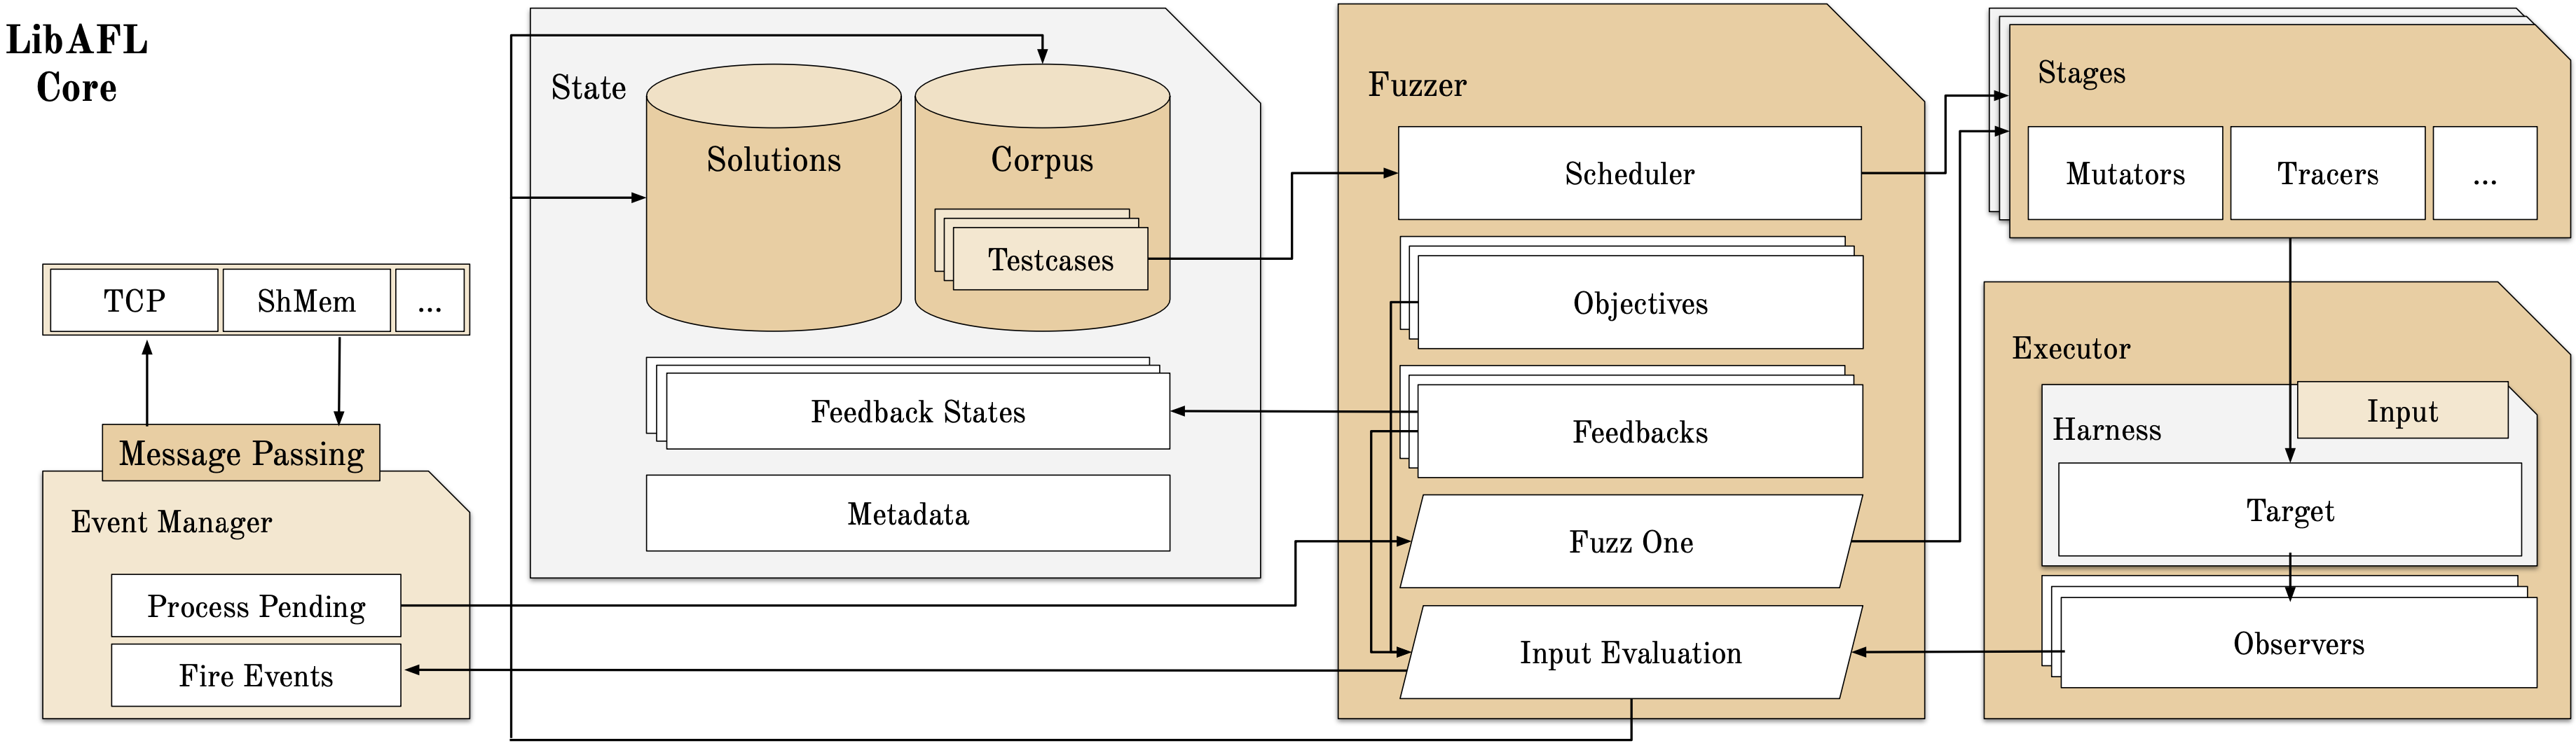
\includegraphics[width=\textwidth]{assets/LibAFLArchitecture.png}
  \caption{LibAFL's Architecture\cite{LibAFL}}
  \label{fig:LibAFLArchitecture}
\end{figure*}

\subsubsection{Central Infrastructure}

The fuzzer relies on \code{CentralizedLauncher} to spawn a number of clients, each with their own data structures and each spawning their own instance of Zephyr. \code{CentralizedLauncher} synchronizes inputs that were added to one of the client's corpi to minimize re-execution and combine the progress made across all clients. Two clients are spawned with a different configuration compared to all other clients: The central synchronizing client does not receive a mutational stage, its only job is synchronization. The last client receives additional feedbacks with constant interestingness-values, which report data about the host system, such as available memory, to the monitor.

Communication between clients is done through Low Level Message Passing (LLMP), a shared memory-based message passing system provided by LibAFL. The absence of a requirement for kernel-based synchronization primitives such as locks allows \proj to effectively scale across thousands of clients.

Central monitoring is configurable in \proj, but defaults to an \code{OnDiskJsonAggregateMonitor}, which will aggregate data across all clients and log it to a machine-readable file. Additionally, a graphical status-board, and a monitor relaying both a client's logs and aggregated logs to the global logging system are provided. LibAFL further supports more complex logging to different data types or other systems such as a prometheus instance, all of which are easily integrated into \proj.

\subsubsection{Client Setup and Operation}
\label{Implementation:ImplementationDetails:Client}

Each client at the start of the fuzzing process initializes its own data structures. These include the following:
\begin{itemize}
  \item A shared memory section to measure coverage in.
  \item A \code{ConstMapObserver} to handle the coverage, wrapped in a \code{HitcountsMapObserver} for binning postprocessing.
  \item A \code{TimeObserver} to measure execution time.
  \item A \code{PacketObserver} responsible for keeping track of transmitted packets, mapping states to a coverage-like map (refer to \cref{Implementation:StateInference}), and providing all required information for the current execution, such as a has of all packets for deduplication of inputs, the states and state-map for debugging purposes, and a base64-encoded packet capture (pcap) representation of the interaction, to allow graphical tools like Wireshark to be used in debugging.
  \item A \code{StdMapObserver} based on the map from the \code{PacketObserver}, to handle state coverage information.
  \item Combined feedback containing
        \begin{itemize}
          \item \code{MaxMapFeedback}s for both code and state coverage information, the only feedbacks contributing values towards the interesting-ness of the current input.
          \item A \code{PacketMetadataFeedback} attaching the metadata provided by the \code{PacketObserver} to the testcase containing the input.
          \item A \code{TimeFeedback}, \code{InputLenFeedback}, and for the last client host system measuring feedbacks, attaching the execution time, input length, and other information to the metadata.
        \end{itemize}
  \item Two corpi: a \code{InMemoryCorpus} for the working corpus of the fuzzer, and an \code{OnDiskCorpus} for all solutions found.
  \item A \code{StdState} containing a random number generator and the corpi.
  \item The appropriate mutators depending on the selected representation of the trace (see \cref{Implementation:InputModelling}).
  \item \code{StdMOptMutator} is used as a mutator scheduler — it implements the algorithm first presented in MOpt\cite{MOpt}.
  \item A \code{StdMutationalStage} wrapping the mutator scheduler and handling the main mutation workflow.
  \item A \code{StdWeightedScheduler} as an input selection scheduler with a power schedule, as known from AFL++\cite{AFLPlusPlus}.
  \item A \code{ReplayingFuzzer} handling the main fuzzing loop — see below for more details.
  \item A custom \code{Executor} implementing all the necessary logic to interact with Zephyr — see below for more details.
\end{itemize}

After setting up all the required data structures, the corpus is filled based on a recorded trace (refer to \cref{Implementation:Seeding}). Because some of the trace subsets result in the same state coverage feedback, but they are still all useful to the fuzzer as starting points from mutations, they are force-generated and afterwards individually evaluated to enhance them with metadata.

Finally, the main fuzzing loop is started. Here, the fuzzer repeatedly calls the scheduler to select the next corpus entry to be mutated. Then, it calls the mutational stage to repeatedly select how many and which mutations to execute on a copy of the input and calls the evaluator in the fuzzer.

Here, the additional logic in \code{ReplayingFuzzer} compared to LibAFL's built-in \code{StdFuzzer} comes into play. It sets up a map to store execution results in, and then repeatedly does the following:
\begin{enumerate}
  \item First, the observers are reset.
  \item Then, the input is passed to the executor to be run.
  \item After that, postprocessing on observers is done.
  \item The results from the observer(s), whose results are to be made more reliable, are hashed and combined with the exit status of the execution.
  \item This combination is then used to index into the execution count map, where \code{ReplayingFuzzer} counts how often each result is measured.
  \item Then, the measurements are evaluated as follows:
        \begin{enumerate}[a.]
          \item If a crash is observed, the fuzzer returns early from the loop to ensure all crashes are caught by the fuzzer.
          \item If the results observed the most have been measured more than a configurable number more often than any other, and the latest execution results in the most common measurements, the execution results are assumed to be "correct" and returned.
          \item If, after a configurable maximum number of executions, the fuzzer is still unable to get a decisive winner, the evaluation is short-circuited and the input is not added to either corpus.
        \end{enumerate}
  \item Finally, the measured ratios are stored and reported to the monitor.
\end{enumerate}

The executor receives the input, and starts its operation by marking the new run in the fuzzing client state and resetting the packet transmission buffers. Then, Zephyr is spawned in a subprocess with the shared memory information for the coverage and network buffer as environment variables. \proj then waits for Zephyr to startup, while logging packets emitted by it, and only responding to those that require a manual response (see \cref{Implementation:NetworkInterface}).

After this interaction, the trace is converted to a list of raw byte vectors to be transmitted to Zephyr. One by one, the packets are sent to Zephyr and added to the \code{PacketObserver}. In between sending packets, \proj waits for Zephyr to respond. Since there is currently no way to wait until Zephyr is done with processing an incoming packet, \proj waits until a set time has expired since the last outgoing or incoming packet. During this phase, manual responses are emitted if appropriate. After the last packet was sent and no packet was received for the set timeout, the subprocess running Zephyr is shut down and checked for a crash to be reported.

There exists a balance between the inter-packet wait time and Zephyr's \code{--rt-ratio} value (see \cref{Implementation:native_sim}) to maximize Zephyr's consistency. If Zephyr is run too quickly, and the inter-packet wait time is set too long, the connection times out before the second packet is sent. In the opposite case, Zephyr may not be done processing a packet before the fuzzer attempts to send the next packet. Initial experiments showed the sweet spot to be at a \code{--rt-ratio} of 1 (thus running Zephyr according to the host's real-time) and an inter-packet wait time of 100ms, interrupted 5 times to check for incoming packets.

\subsubsection{Helper Functionality}
\label{Implementation:ImplementationDetails:HelperFunctionality}
\proj contains additional logic helpful during development and triage of found issues. First, an implementation of the shared memory-based ethernet driver for the userland network client \code{smoltcp} allows manual interaction with Zephyr through shared memory. Additionally, a set of postprocessing scripts are available, which, among other things, extract pcap files from the corpus, and produce plots as shown in \cref{Results}.

\subsection{Contributions to LibAFL}
\label{Implementation:ContributionsToLibAFL}

During this project, I have contributed a range of improvements implemented for \proj as generic version to LibAFL. These include:
\begin{itemize}
  \item \code{MappingMutator}s are essential for any project using compound input types — they allow mapping mutators targeting a certain type to those where the initial input type can be extracted from using custom logic. One such example would be applying \code{havoc_mutations} to the payload field of the TCP packet.\footnote{Currently, only non-crossover mutations are supported in \proj, because of a limitation in LibAFL with using nested \code{MappingMutator}s. This is required to map mutators from their raw target type (such as byte array or number) to the parsed input structure and then again to the composite type such as \code{ListInput}.}
  \item \code{CentralizedLauncherBuilder::overcommit} and \code{LauncherBuilder::overcommit} allows users to launch multiple fuzzing clients per CPU core. This is useful in specific projects like \proj, where an individual client does not fully load a CPU core because of wait states necessary for e.g. synchronization.
  \item \code{int_mutators} include the applicable mutators from \code{havoc_mutations} targeting numeric types.
  \item \code{BoolMutator}s flip boolean values.
  \item \code{ValueInput}, an improvement to how inputs encapsuling a simple data type are implemented.
  \item A set of macros for mapping and combining mutator lists and their types.
  \item Improved flexibility for certain schedulers to work on any observer.
  \item \code{OnDiskJsonAggregateMonitor} logs the data aggregated across all fuzzing clients at a certain interval to a file containing machine-readable data.
  \item Several bugfixes related to \code{MultipartInput}.
  \item Several general architectural and clean-code improvements.
  \item An adaptation of \code{ListInput}, including additional mutators.\todo{Change depending on results of the PR}
  \item \code{StdFuzzer::with_bloom_input_filter}, an improvement to \code{StdFuzzer} which uses a probabilistic filter to reduce repeated execution of the same input\footnote{Not currently used in \proj.}
\end{itemize}

%%%%%%%%%%%%%%%%%%%%%%%%%%%%%%%%%
%%% Evaluation & Results %%%%%%%%
%%%%%%%%%%%%%%%%%%%%%%%%%%%%%%%%%

\section{Evaluation and Results}
\label{Results}

\todo{@Peter do I need explicit research questions here? Or is this clear by the headings and what I set up in the text (here and before)?}

\proj was evaluated along multiple axis, starting with experiments on the consistency of the target, and then evaluating the effectiveness of the different improvements implemented in \proj.

All experiments were performed on a 64-core AMD EPYC-Milan machine, using the configuration and parameters described in \cref{Implementation} unless indicated otherwise.

\subsection{Consistency}
\label{Results:Consistency}
To evaluate the consistency of the PUT when executed by the fuzzer, I changed \proj to use \code{StdScheduler}, which selects inputs from the corpus at random, to generate a wider range of inputs. I further set up \code{ReplayingFuzzer} to evaluate input traces until the most common appears at least 100 times and a factor of 1.5 more often than any other input, up to 1500 executions per input.

When \proj is setup to use both coverage and state-diff feedback, and requiring inputs to be consistent in both their coverage and state measurements, the results in \cref{fig:both-inter} are measured. The results for runs checking coverage and state-diff feedback exclusively can be found in \cref{fig:cov-inter,fig:state-diff-inter}. All figures show the average stability measured across trace lengths. The evaluations were run across 64 cores, with 10 clients per core, for approximately 24 hours and 40 million target executions on individual feedbacks, and for 48 hours for the combined feedback.

\todo{Re-render plots at higher DPI, fix placement}
\begin{figure}
  \makebox[\columnwidth]{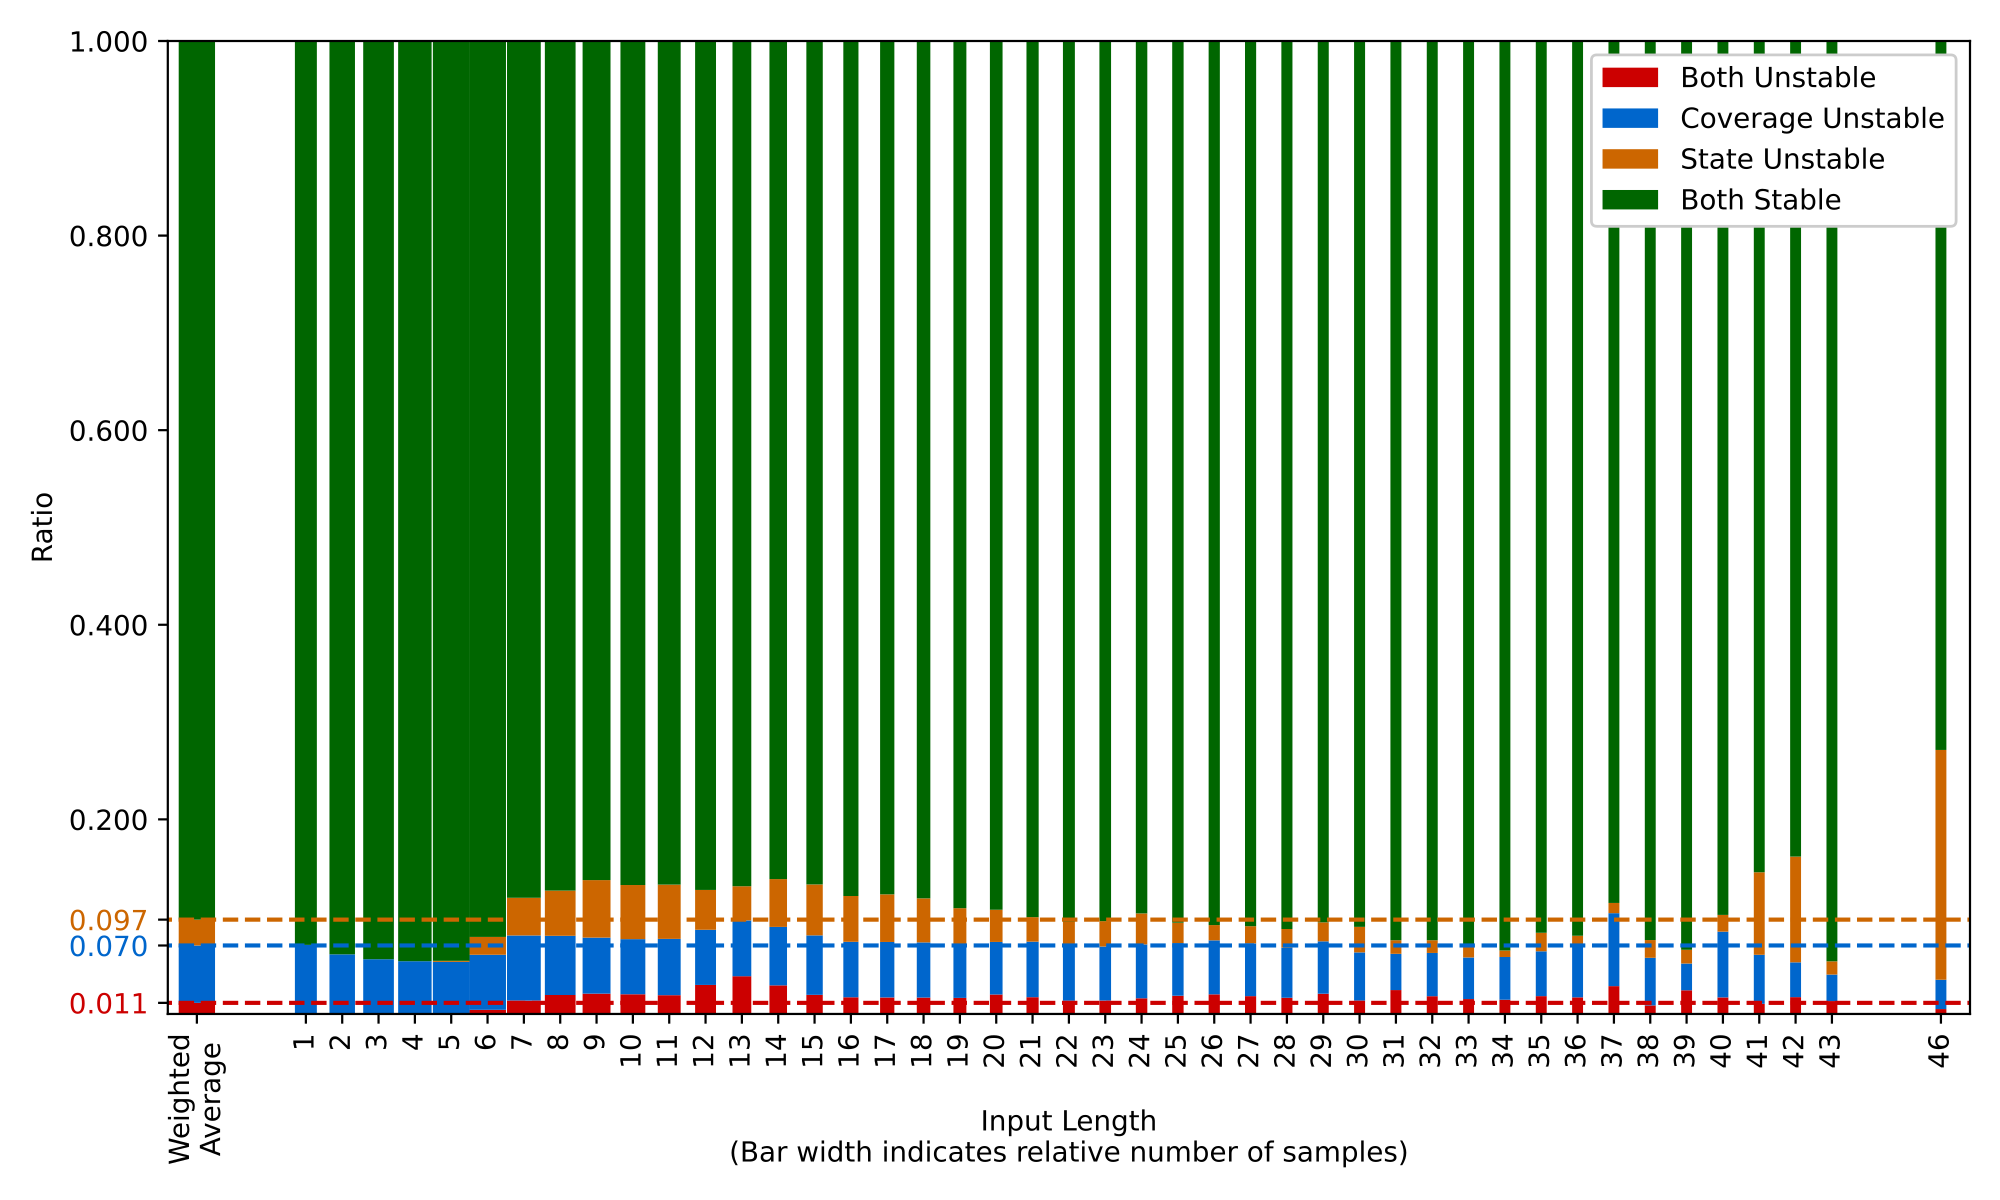
\includegraphics[width=1.1\columnwidth]{assets/consistency/both-observer-ratios-by-len.png}}
  \caption{Average stability of both feedbacks across trace lengths}
  \label{fig:both-inter}
\end{figure}
\begin{figure}
  \makebox[\columnwidth]{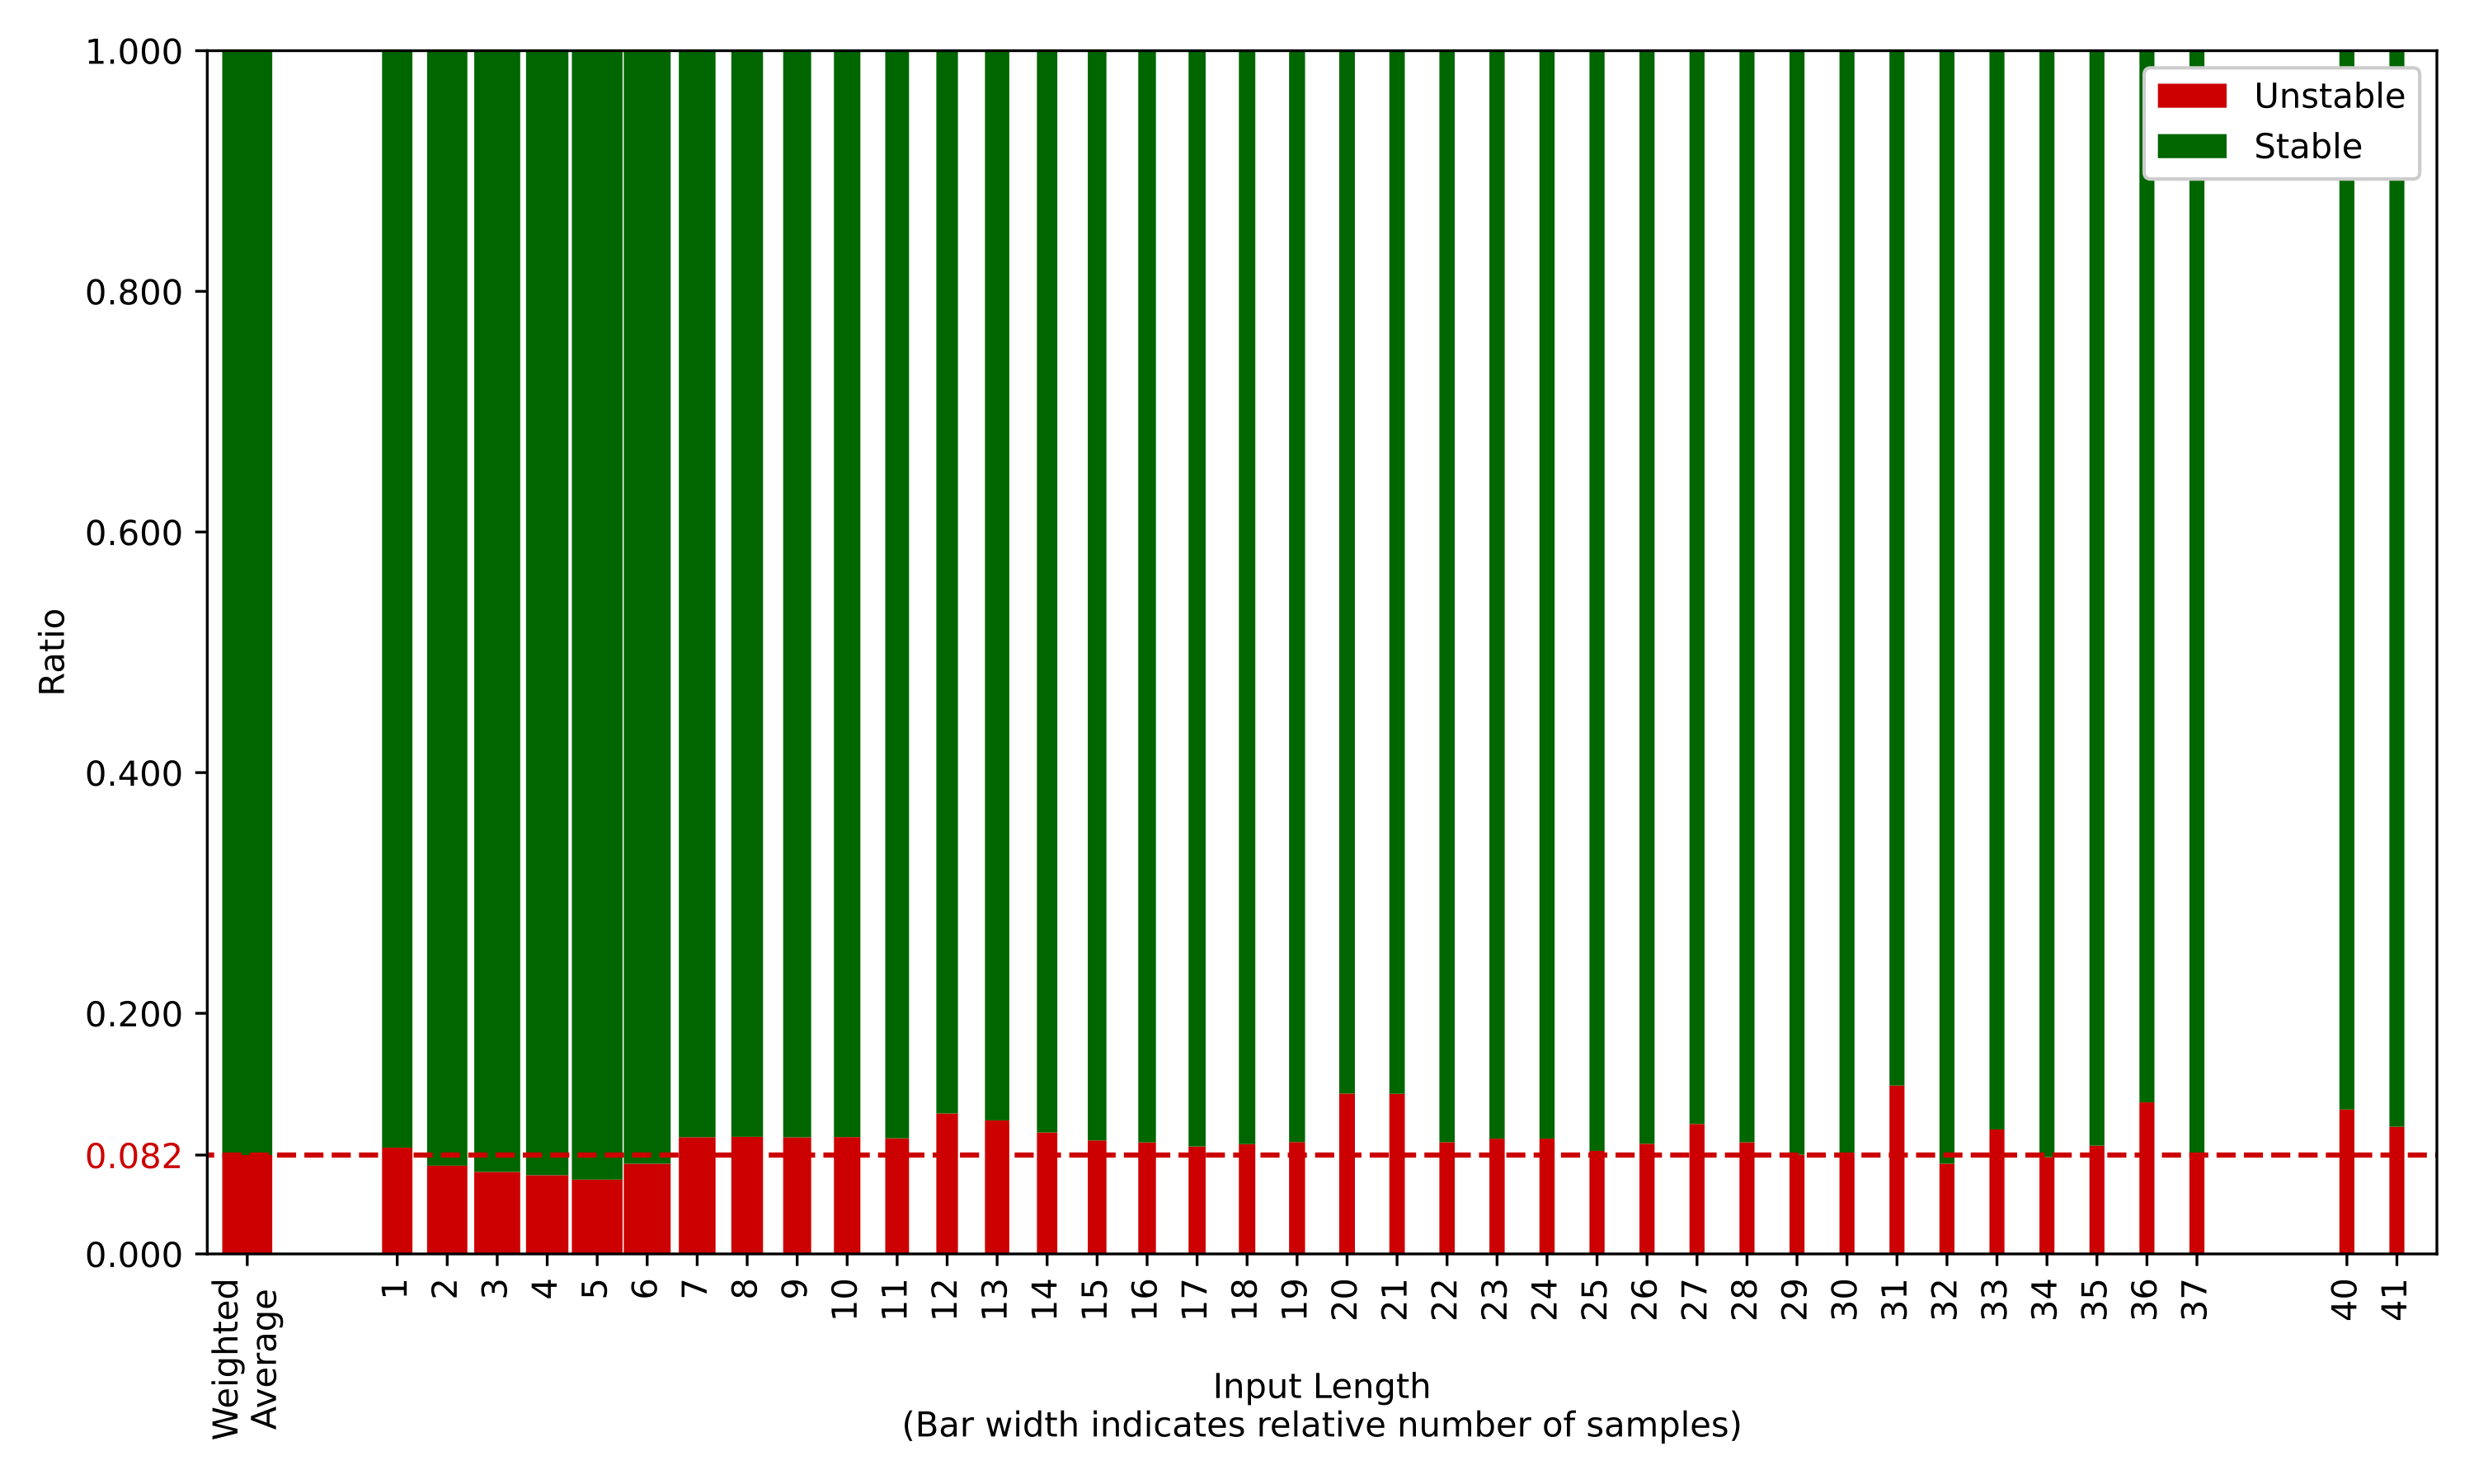
\includegraphics[width=1.1\columnwidth]{assets/consistency/coverage-observer-ratios-by-len.png}}
  \caption{Average stability of coverage feedback across trace lengths}
  \label{fig:cov-inter}
\end{figure}
\begin{figure}
  \makebox[\columnwidth]{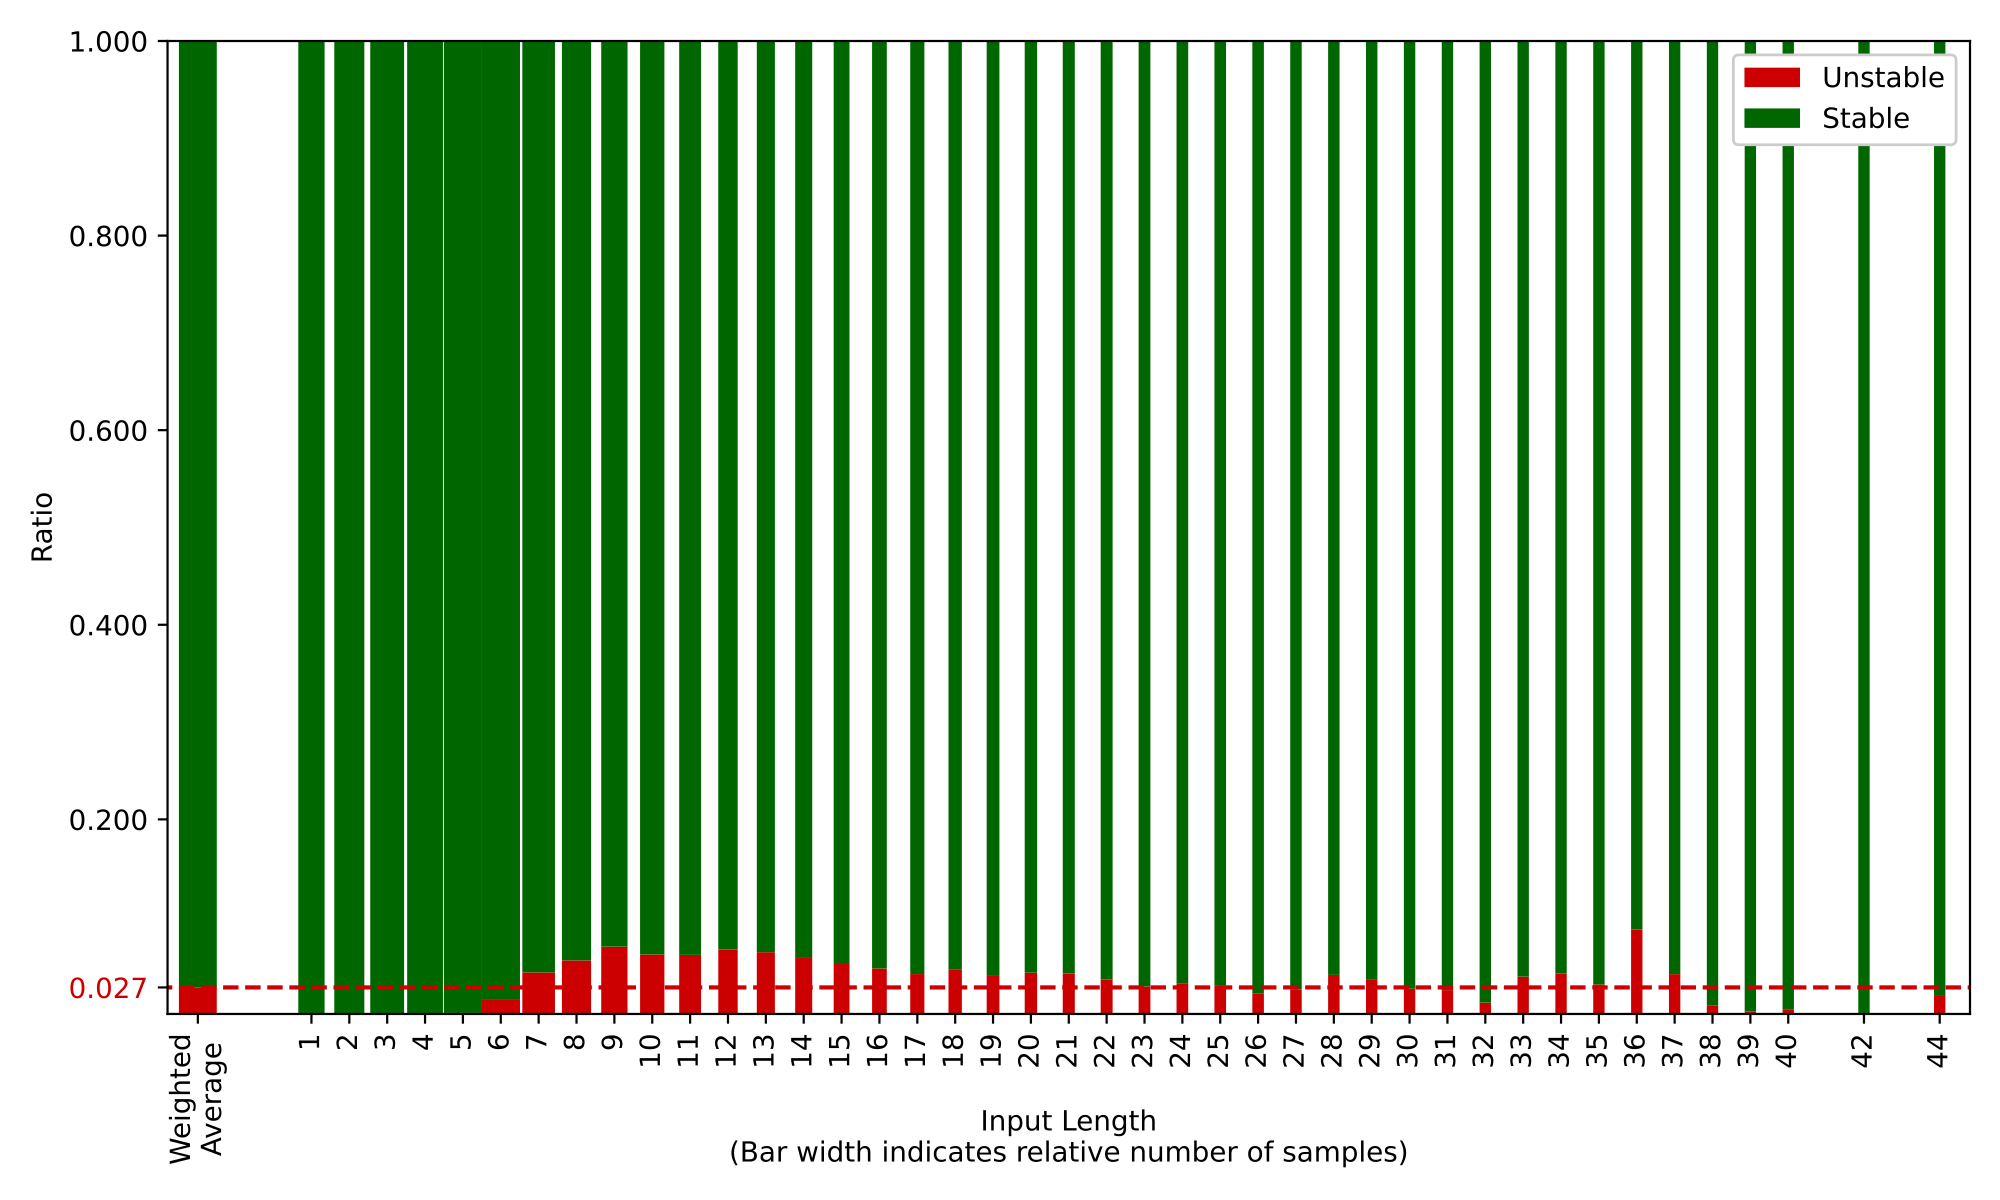
\includegraphics[width=1.1\columnwidth]{assets/consistency/state-diff-observer-ratios-by-len.png}}
  \caption{Average stability of state-diff feedback across trace lengths}
  \label{fig:state-diff-inter}
\end{figure}

To find the source of the different coverage maps measured across multiple executions of the same input, I added additional logging to \code{__sanitier_cov_trace_pc_guard} (refer to \cref{Implementation:SanCov}), recording the guard index and the address the function returns to. The latter is used to map guard to source code location. At the same time, the differences between executions are mapped back to guard index in the fuzzer and recorded. This information is then combined, and sorted by how often each guard appears. The most common functions appearing in this list are the following:
\begin{enumerate}
  \item \code{k_work_init_delayable} from \code{kernel/work.c}
  \item \code{net_ipv6_mld_init} from \code{net/ip/ipv6_mld.c}
  \item \code{sys_slist_init} from \code{sys/slist.h}
  \item \code{z_slist_tail_set} from \code{sys/slist.h}
  \item \code{net_conn_init} from \code{net/ip/connection.c}
\end{enumerate}

Further notable entries include \code{net_ipv4_init}, \code{net_tcp_init}, and \code{net_init}. Across 137,571 executions of Zephyr, differences at 232,903 offsets in the coverage map were measured, the most common (\code{k_work_init_delayable}) appeared in 1745 executions, 73 of 386 entries found to not always be consistent appeared in fewer than 0.1\% of all executions.

\subsubsection*{Discussion}
Both coverage and state-diff results show inconsistencies when Zephyr is run by \proj.

\begin{figure*}[p]
  \centering
  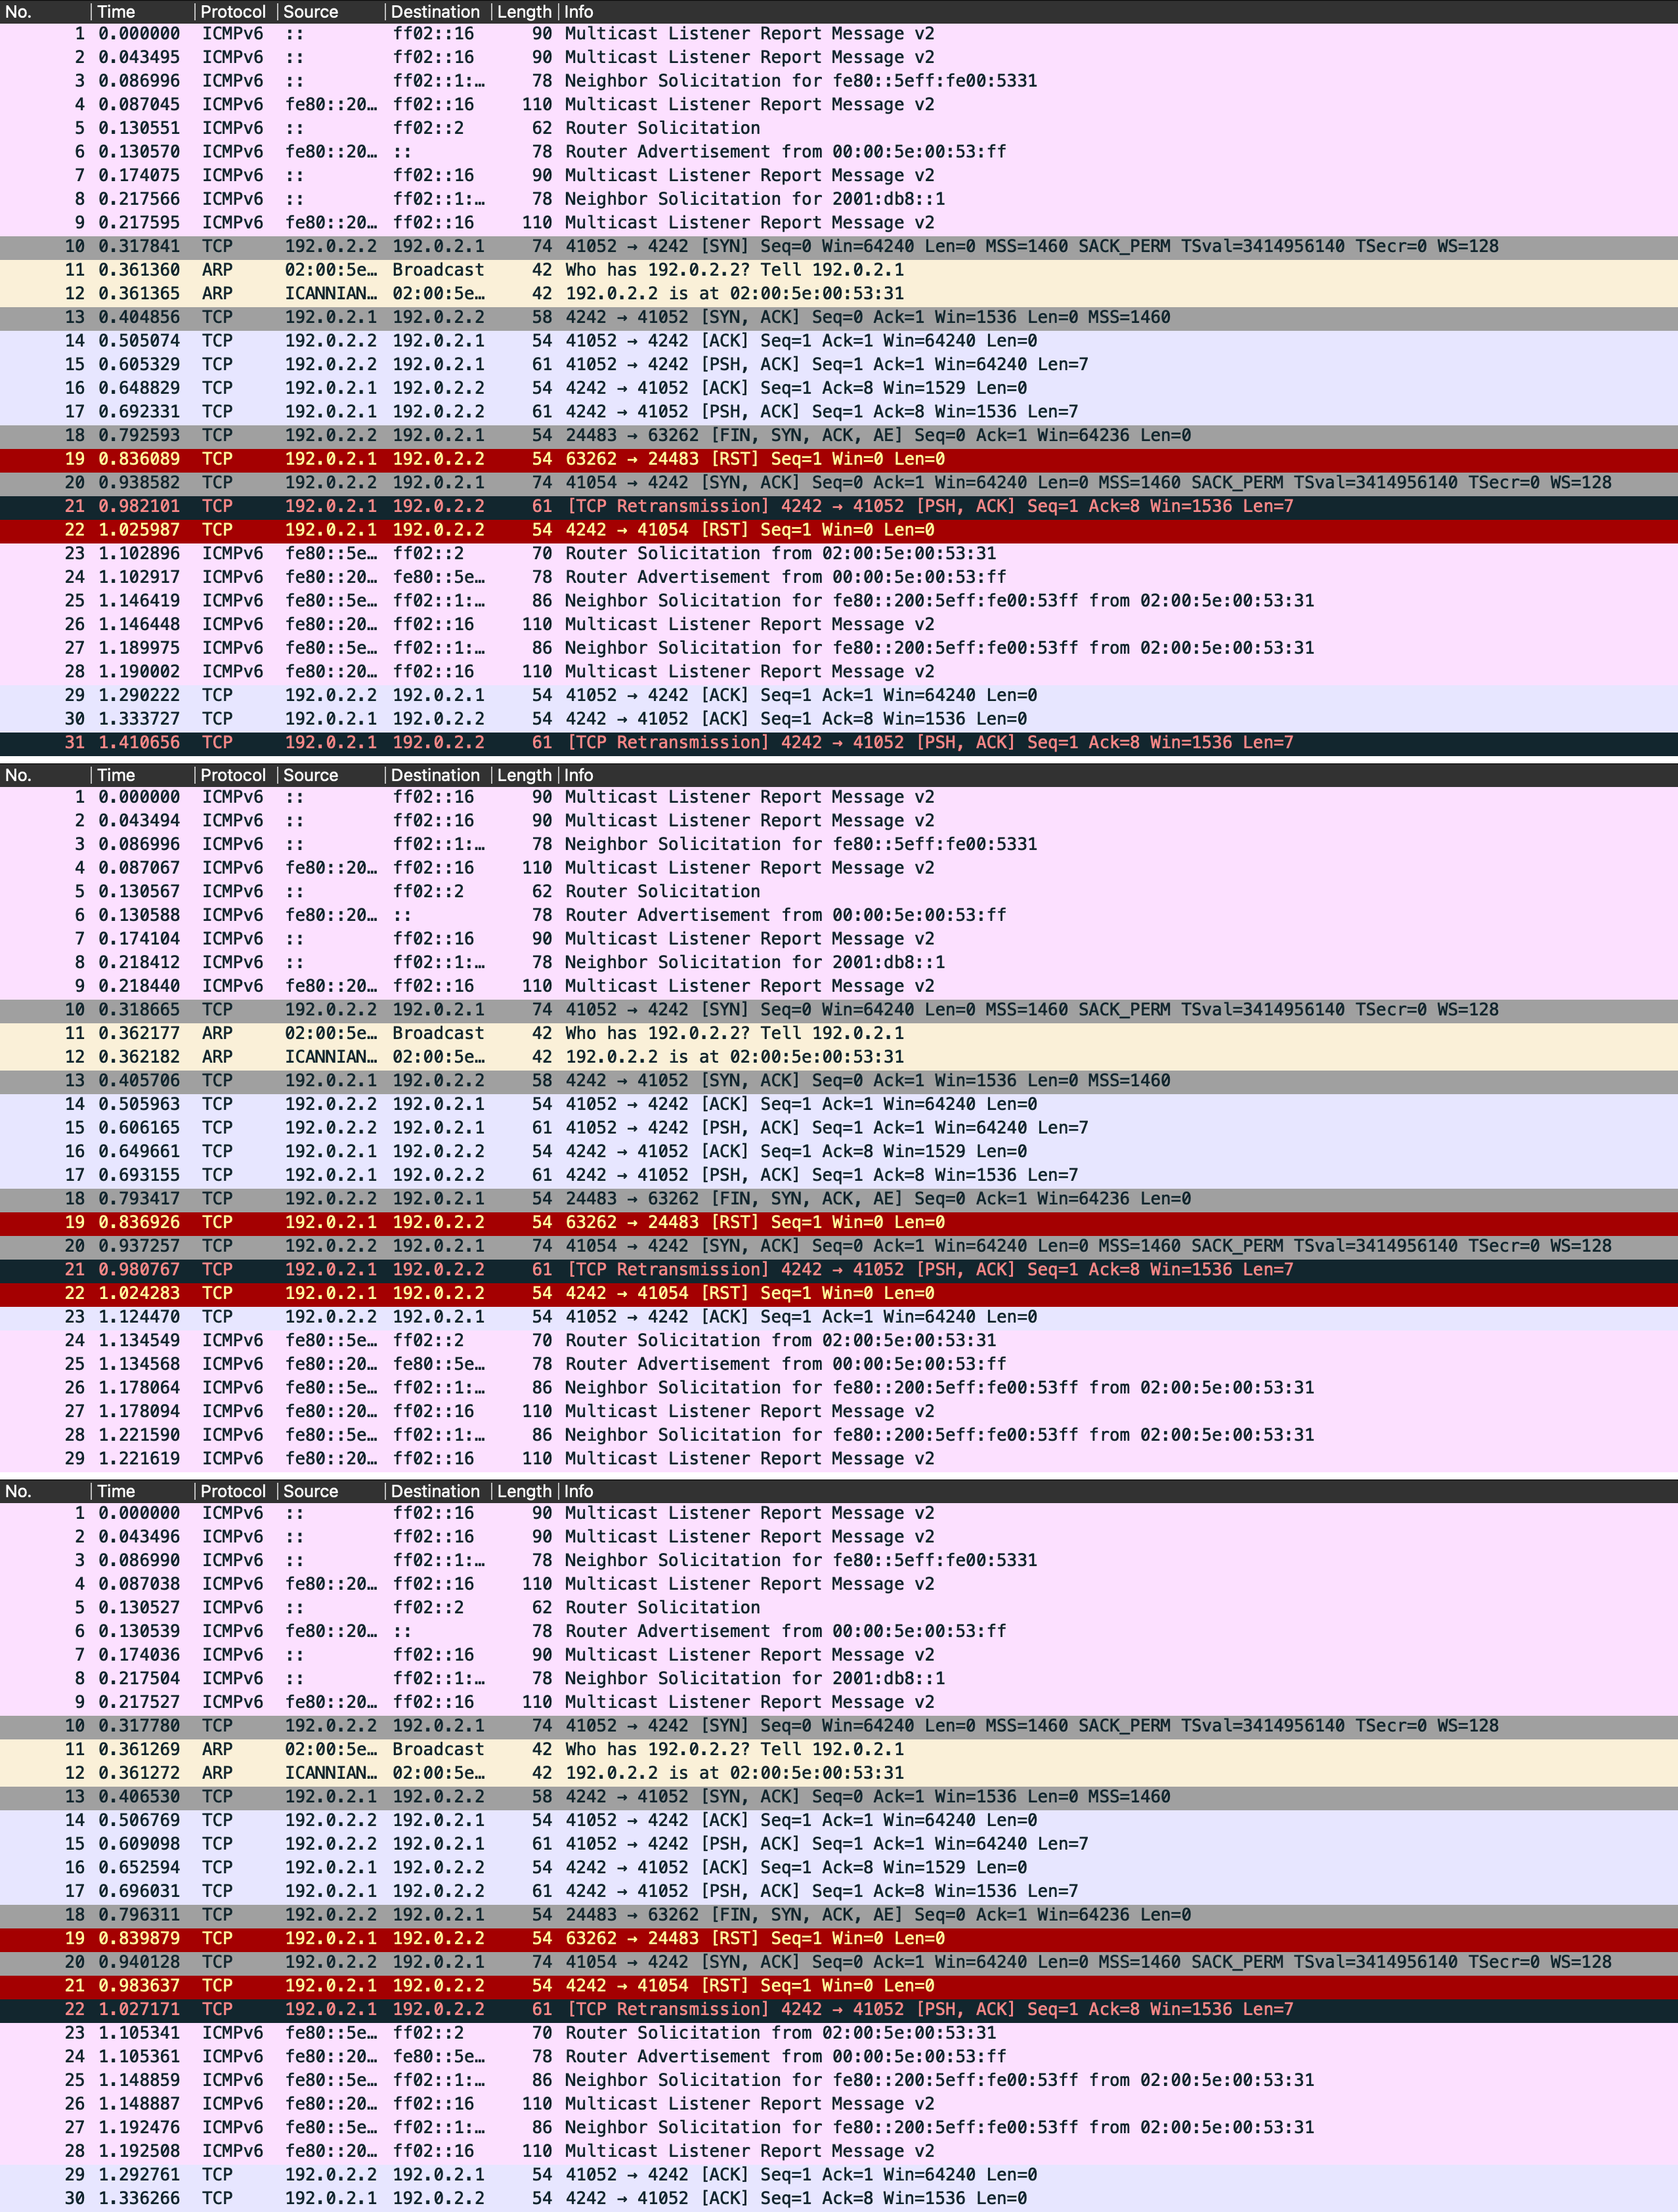
\includegraphics[width=0.95\textwidth]{assets/consistency/wireshark-combined.png}
  \caption{Packets exchanged for the same input in 10 executions, recorded 4, 4, and 2 times respectively}
  \label{fig:wireshark-combined}
\end{figure*}
\paragraph{Distribution}

\paragraph{Coverage}
As discussed in \cref{Implementation:SanCov}, for certain coverage entries, \textit{how often} a certain basic block is executed is expected to be inconsistent because of inherent inconsistencies of the non-deterministic host scheduler. However, since \proj only taints executed basic blocks, the differences measured are between a basic block being executed any number of times and the basic block not being executed at all. Functions such as \code{net_init} should be called on every launch, and if they are not executed, Zephyr may not be initialized correctly, thus invalidating any evaluation on it, indicating that the differences in coverage can not be ignored by \proj. It is further notable that many of the functions in the list of inconsistently executed basic blocks appear to be related to system startup and initialization. Finally, coverage is measured with high consistency across trace length, which may suggest that the logic only executed sometimes is not related to packet handling.

While \cref{Results:Overcommit} explores how different configurations of Zephyr make both state and code coverage less stable at the host's performance limit, I was unable to determine the fundamental source of these inconsistencies. Because of the high rate of inconsistency in the measurements of basic block coverage, I decided to not use it as feedback to the fuzzer in \proj. However, the values can still be used as a heuristic to measure the fuzzer's ability to test all system parts recorded at any part in any execution. Since \code{MaxMapFeedback} records map entries present in \textit{any} map passed to it, even if a certain function is not called in one execution because something went wrong, e.g. during Zephyr's initialization logic, the same function is likely to be triggered in one of the other executions.

\paragraph{State-Diff}

The differences as measured by the state-diff observer indicates a difference in packets received by the fuzzer. This could be confirmed by manual inspection of the different interactions between the fuzzer and Zephyr from the same input. As described in \cref{Implementation:ImplementationDetails:HelperFunctionality,Implementation:ImplementationDetails:Client}, \proj provides functionality to extract these into \code{pcap} files. \cref{fig:wireshark-combined} shows screenshots of three different exchanges recorded for 10 executions with the same input.

Like in the example, retransmitted packets and those resetting the connection appear frequently. However, I was unable to find a reason for the inconsistencies or a definite pattern between them.

Unlike with basic block coverage, state-diff coverage seems to be trace-length dependent: Traces with length $\le5$ are almost always consistent with respect to the packets exchanged between fuzzer and Zephyr. However, the ratio does not continue rising with increased trace length after that, as would be expected if the error rate is independent of state and packet. This suggests that there remains an unknown factor influencing reliability of Zephyr's responses. The fact that short traces are executed comparatively consistently may be caused by either a filling buffer in Zephyr or an underlying problem requiring Zephyr to be in a state only reachable with a certain number of packets.

\paragraph{Distribution}

% The consistencies of both feedbacks show a further notable statistic: The average incorrect-to-correct ratios are higher than the medians by a considerable margin across all trace lengths (at least for those that have a significant number of traces evaluated). \cref{fig:both-inter-boxplot,fig:cov-inter-boxplot,fig:state-diff-inter-boxplot} show the distribution of ratios between the incorrect and correct measurements across trace lengths. For an input that provoked three different observer values appearing 2, 10, and 100 times, this ratio would therefore be 0.12. This conjecture is further compounded for state-diff feedback specifically by the distribution of the ratios according to \cref{fig:state-diff-inter-violin}, showing two sections along the y-axis with higher densities, at approximately 0.1 and 0.75 respectively, with fewer inputs resulting in consistencies at around 0.4. These distributions may be used to further evaluate whether either one or both feedbacks behave inconsistent for all inputs equally or if there exists a class of inputs for which Zephyr behaves more or less consistently. However, I was unable to complete an in-depth evaluation of this phenomenon as part of this thesis.

The consistencies of both feedbacks show a further notable statistic: There seems to be a set of inputs triggering inconsistent behavior more likely than others. \cref{fig:state-diff-inter-violin} shows the distribution of ratios between the incorrect and correct measurements across trace lengths. For an input that provoked three different observer values appearing 2, 10, and 100 times, this ratio would therefore be 0.12. There appear two sections along the y-axis with higher densities, at approximately 0.1 and 0.75 respectively, with fewer inputs resulting in consistencies at around 0.4. However, I was unable to complete an in-depth evaluation of this phenomenon as part of this thesis.

% \begin{figure}
%   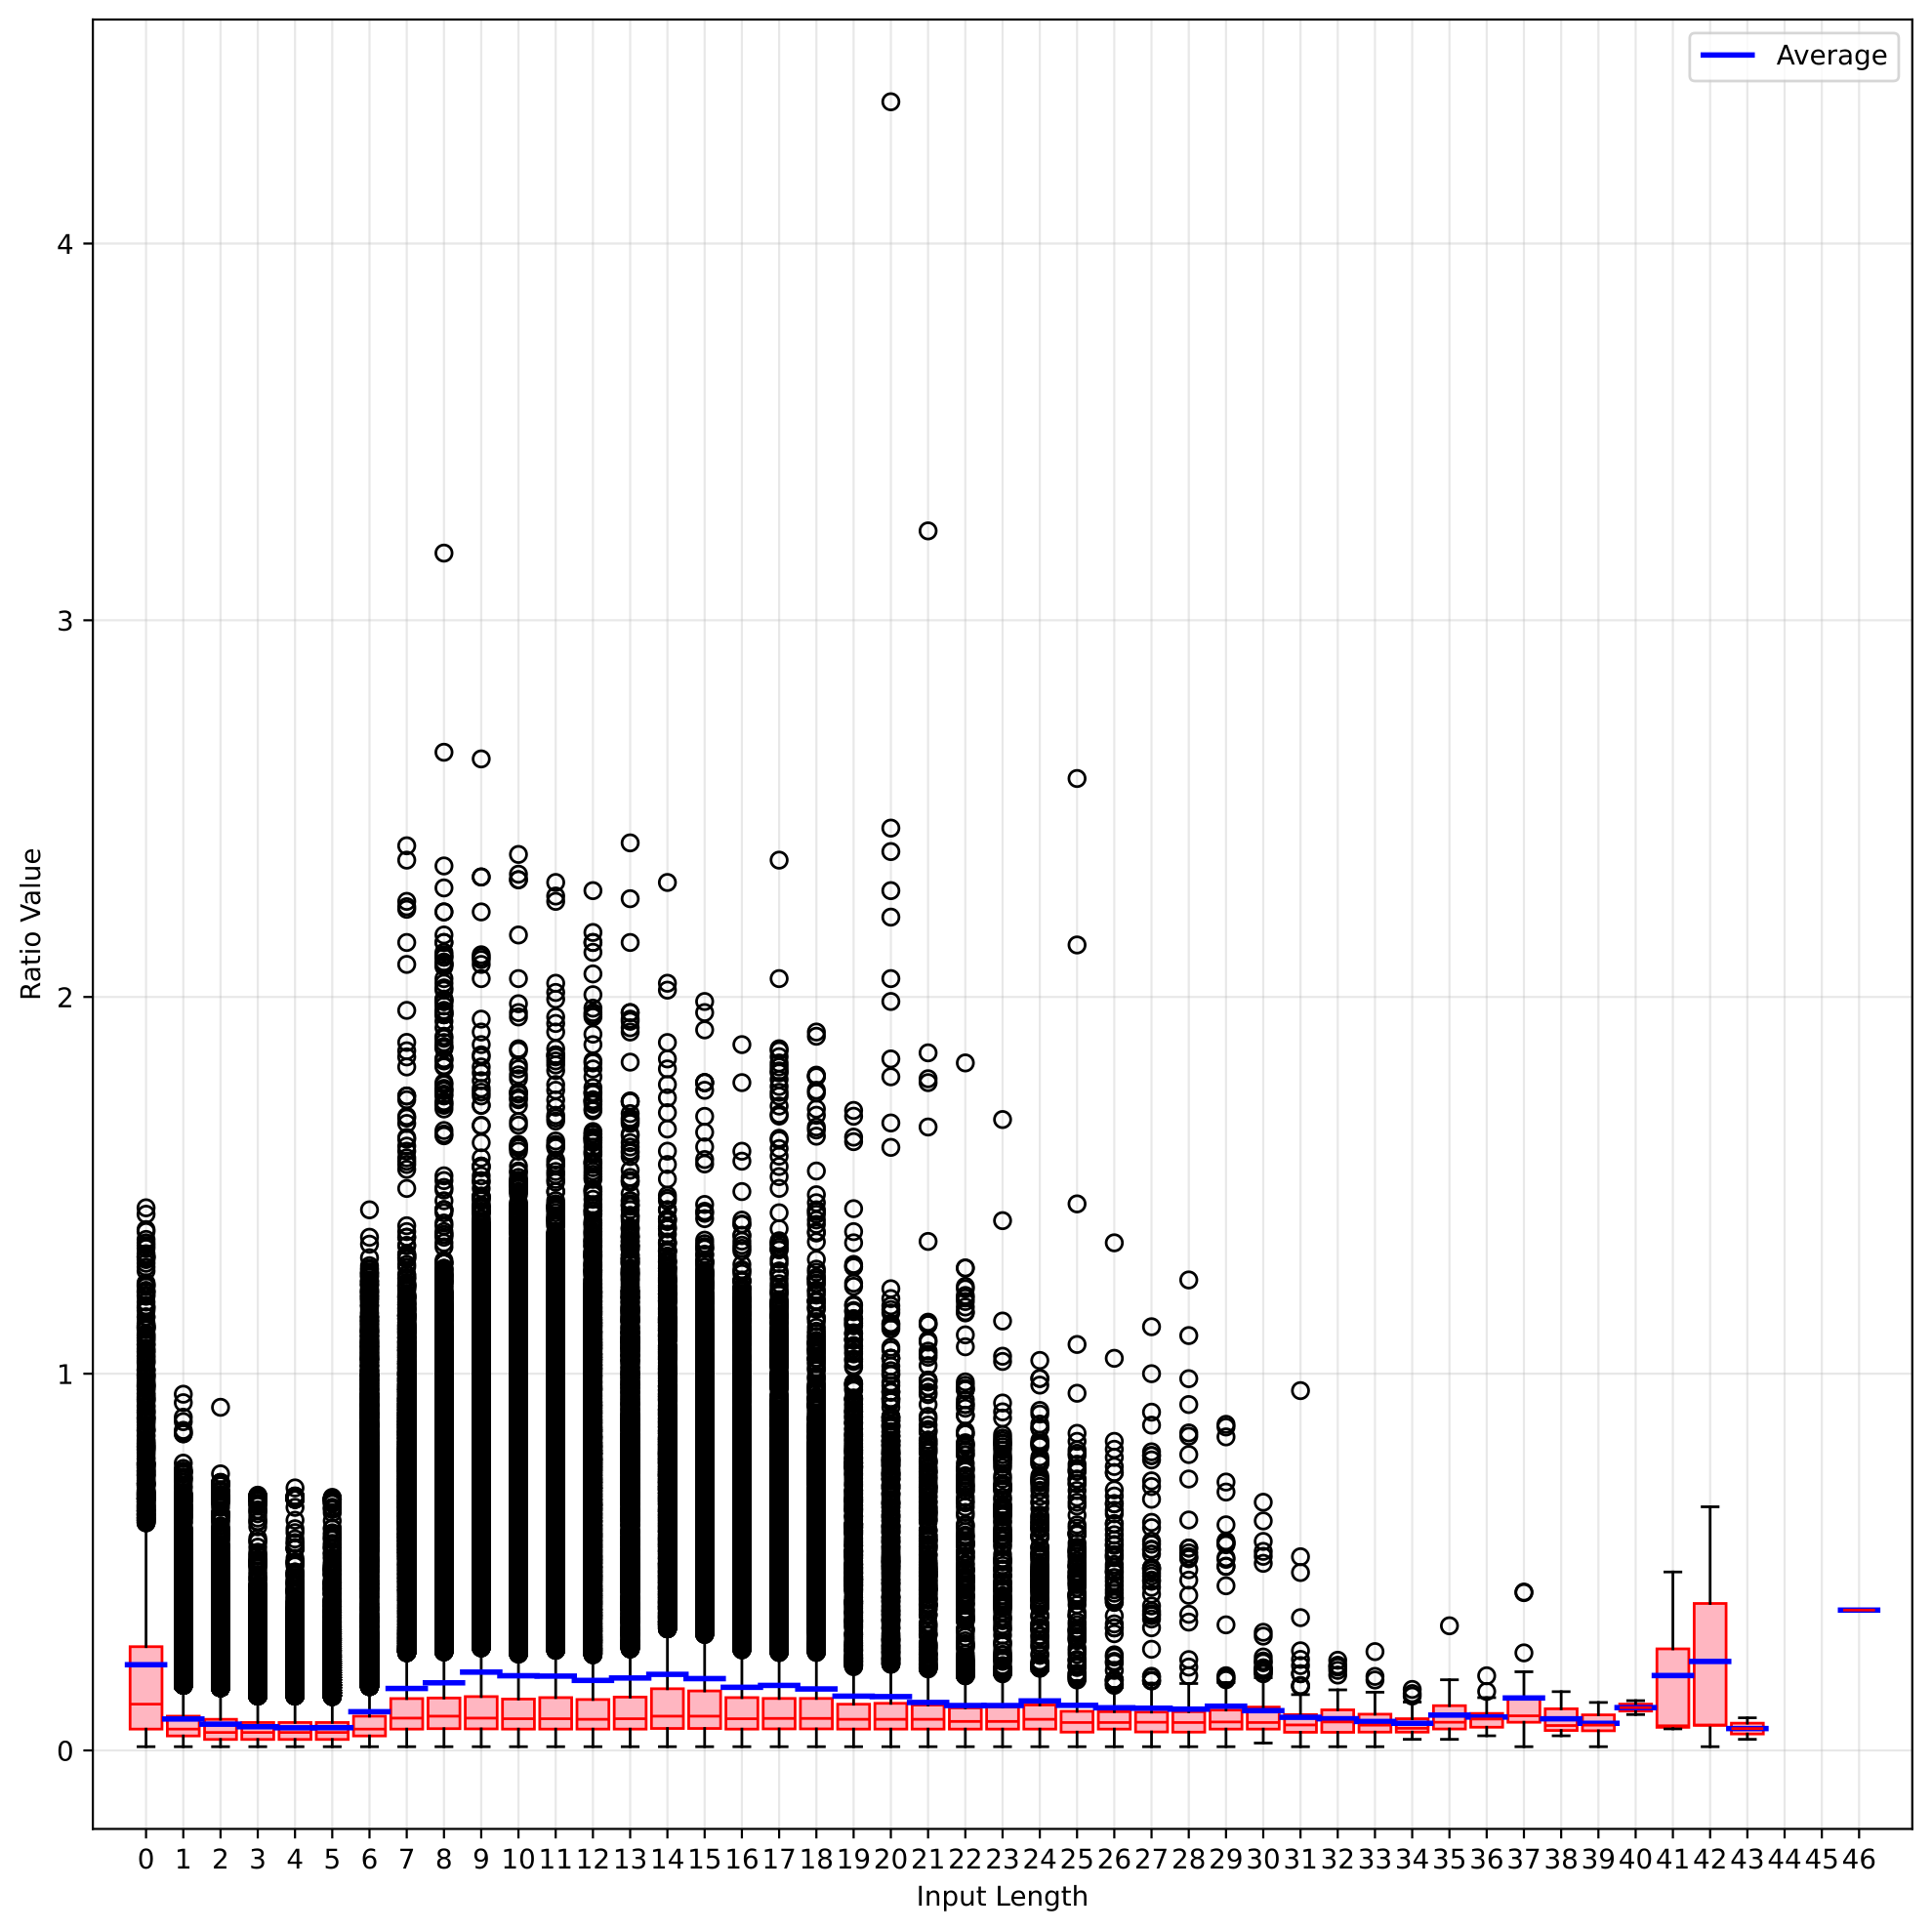
\includegraphics[width=\columnwidth]{assets/consistency/both-boxplot.png}
%   \caption{Ratio between incorrect and correct observer measurements across trace lengths when using both feedbacks}
%   \label{fig:both-inter-boxplot}
% \end{figure}
% \begin{figure}
%   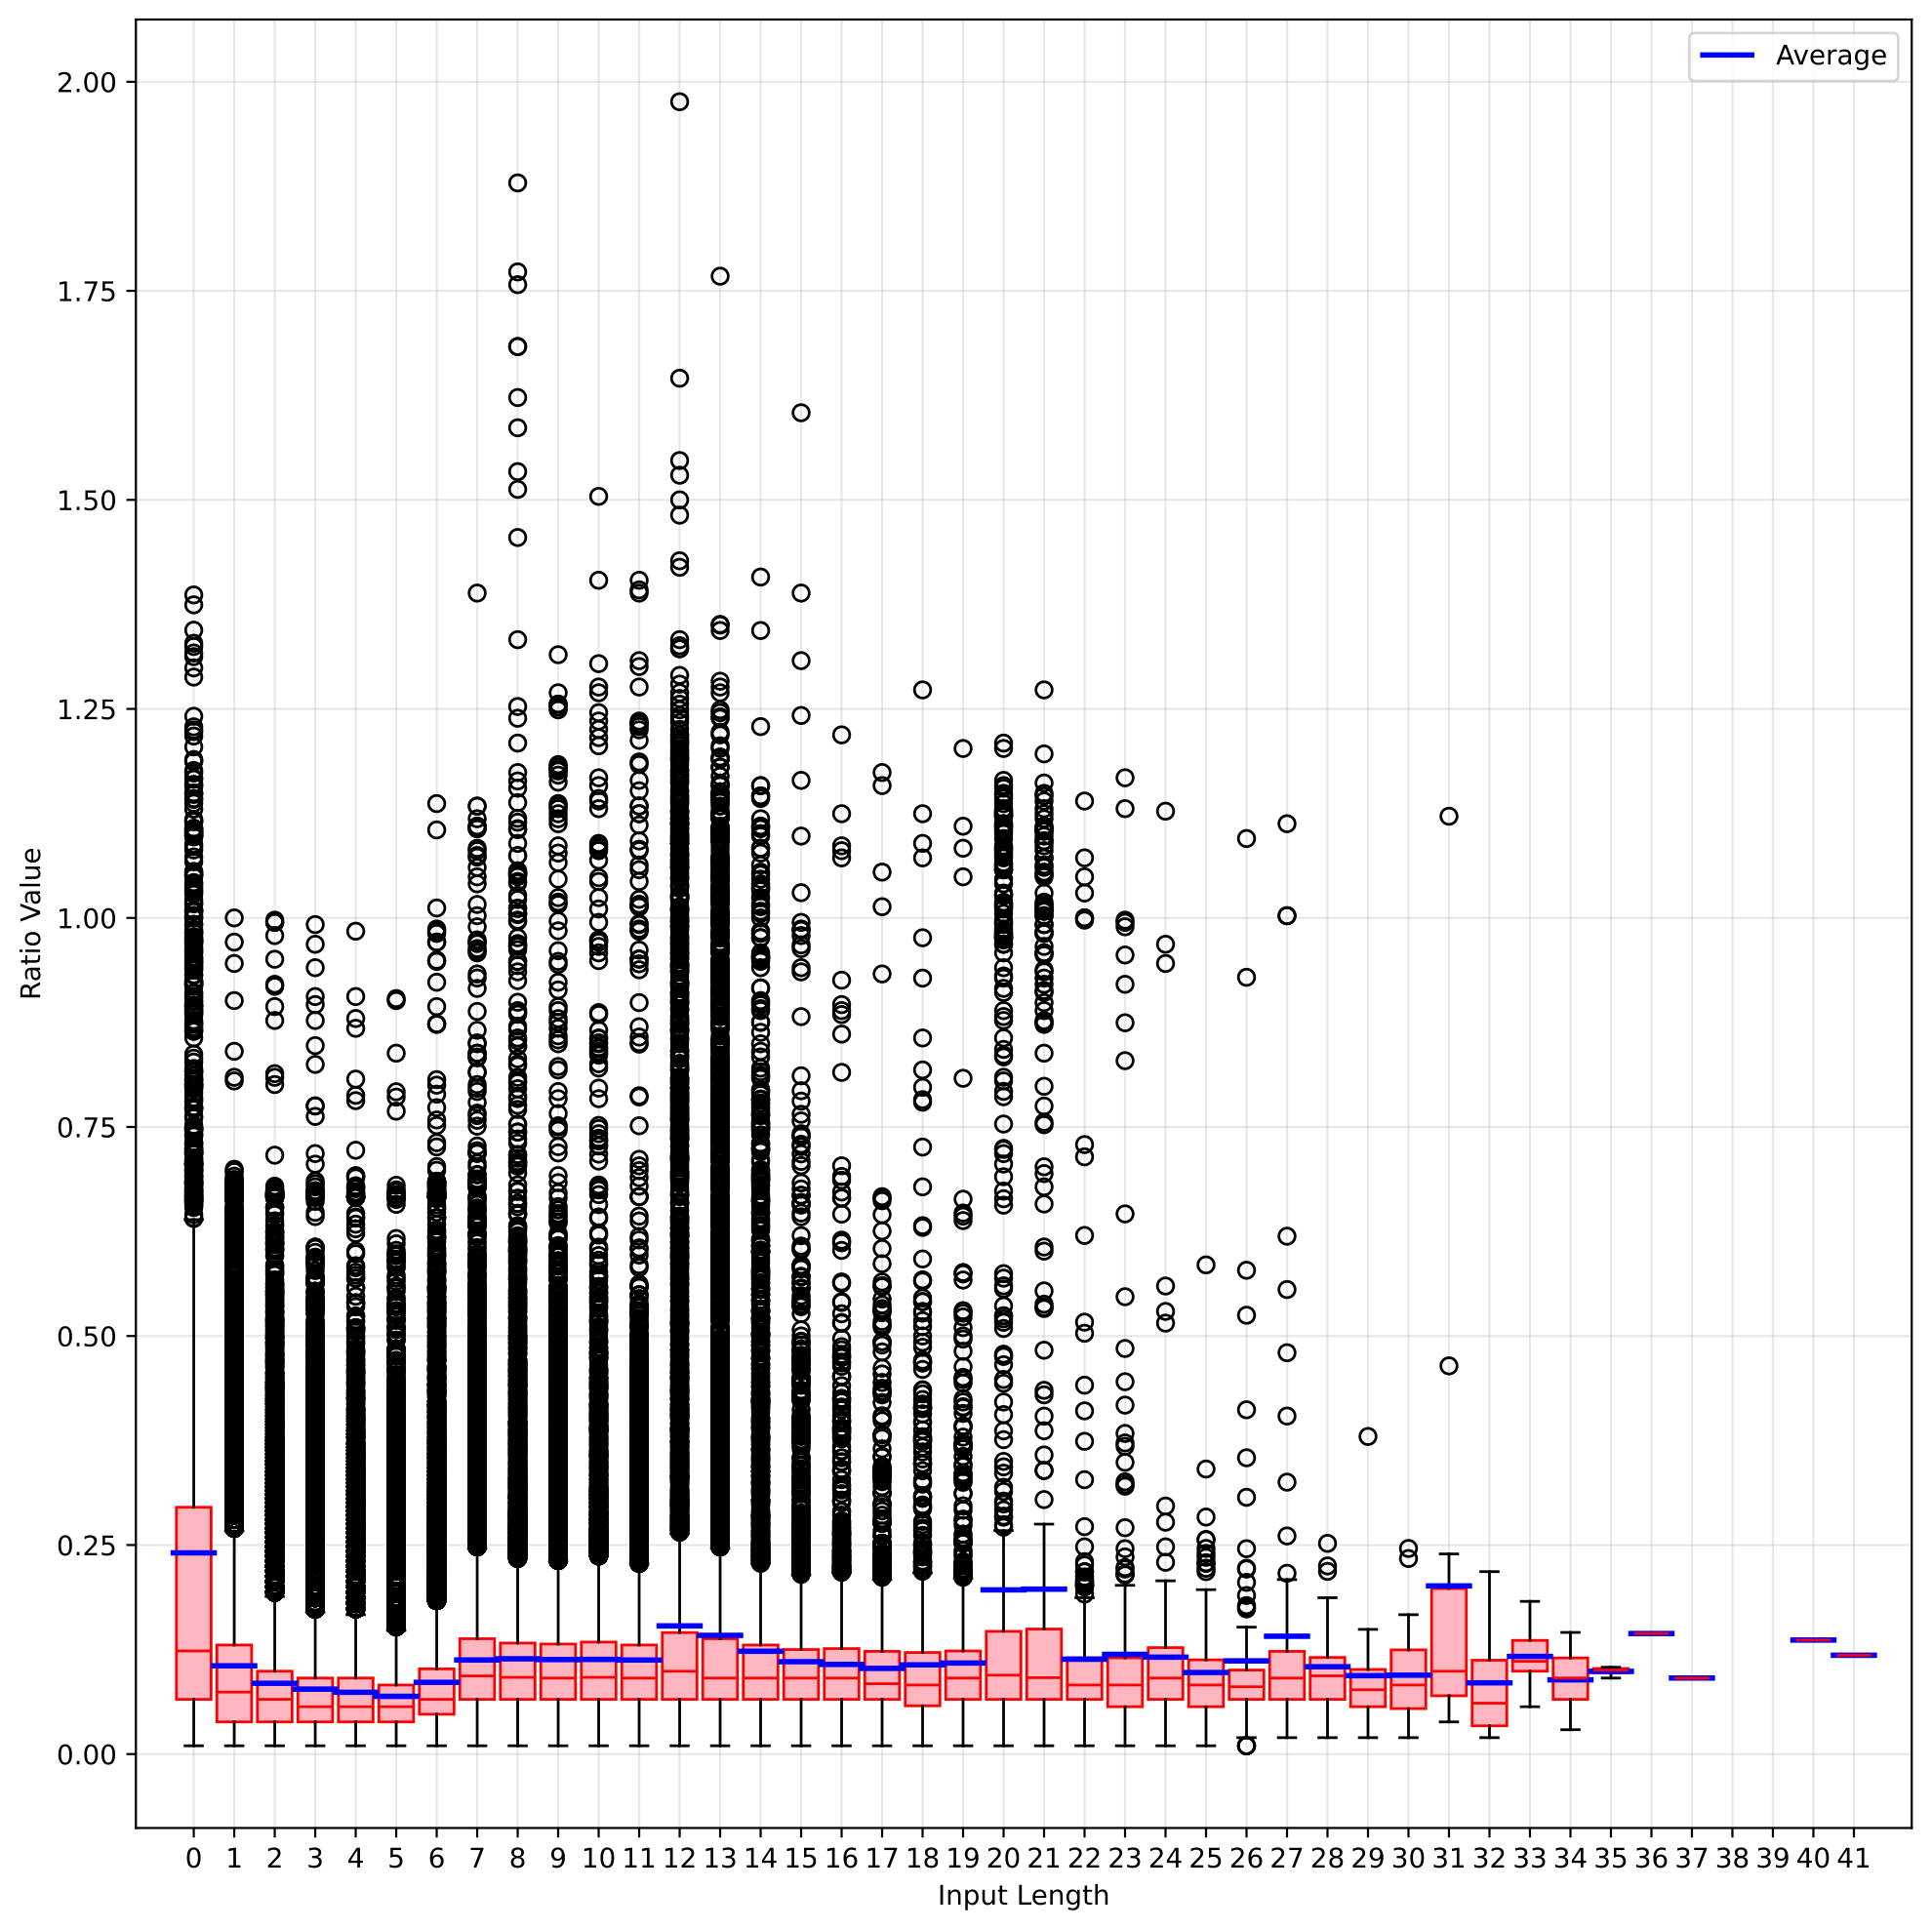
\includegraphics[width=\columnwidth]{assets/consistency/coverage-boxplot.png}
%   \caption{Ratio between incorrect and correct observer measurements across trace lengths when using coverage feedback}
%   \label{fig:cov-inter-boxplot}
% \end{figure}
% \begin{figure}
%   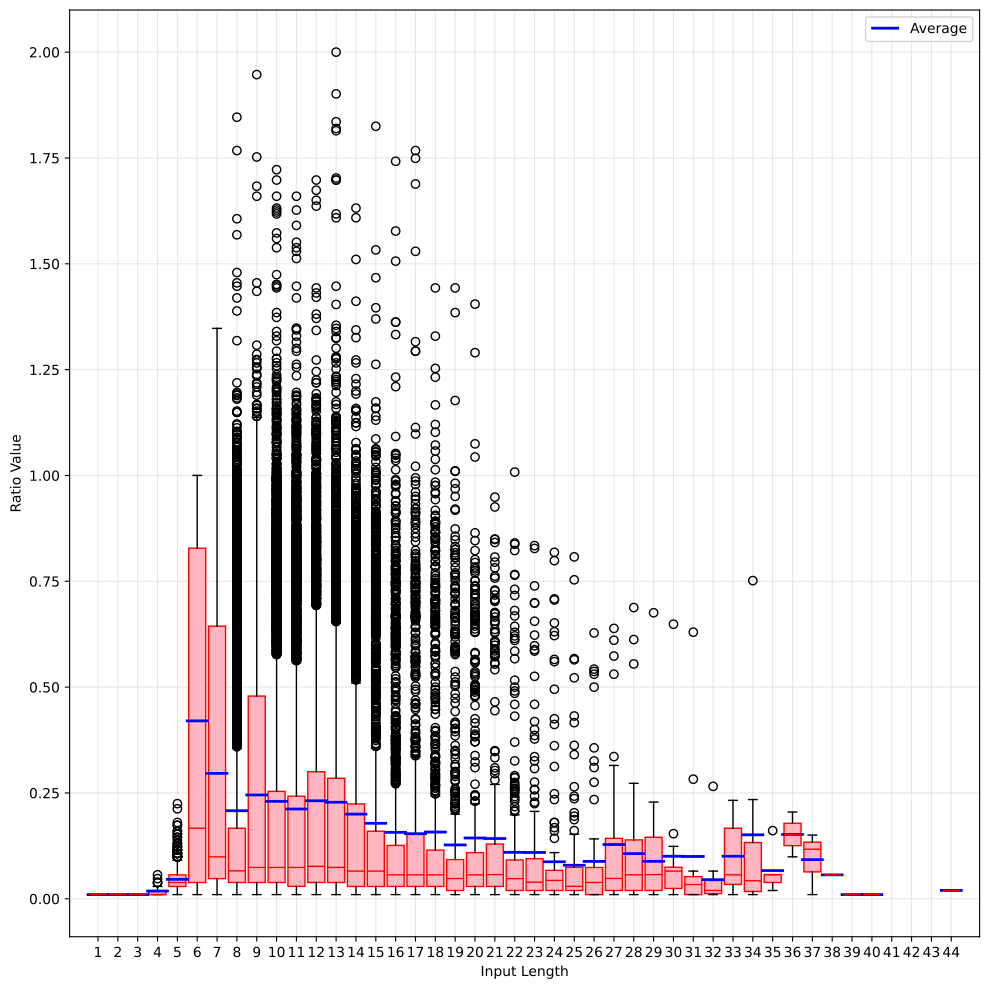
\includegraphics[width=\columnwidth]{assets/consistency/state-diff-boxplot.png}
%   \caption{Ratio between incorrect and correct observer measurements across trace lengths when using state-diff feedback}
%   \label{fig:state-diff-inter-boxplot}
% \end{figure}
\begin{figure}
  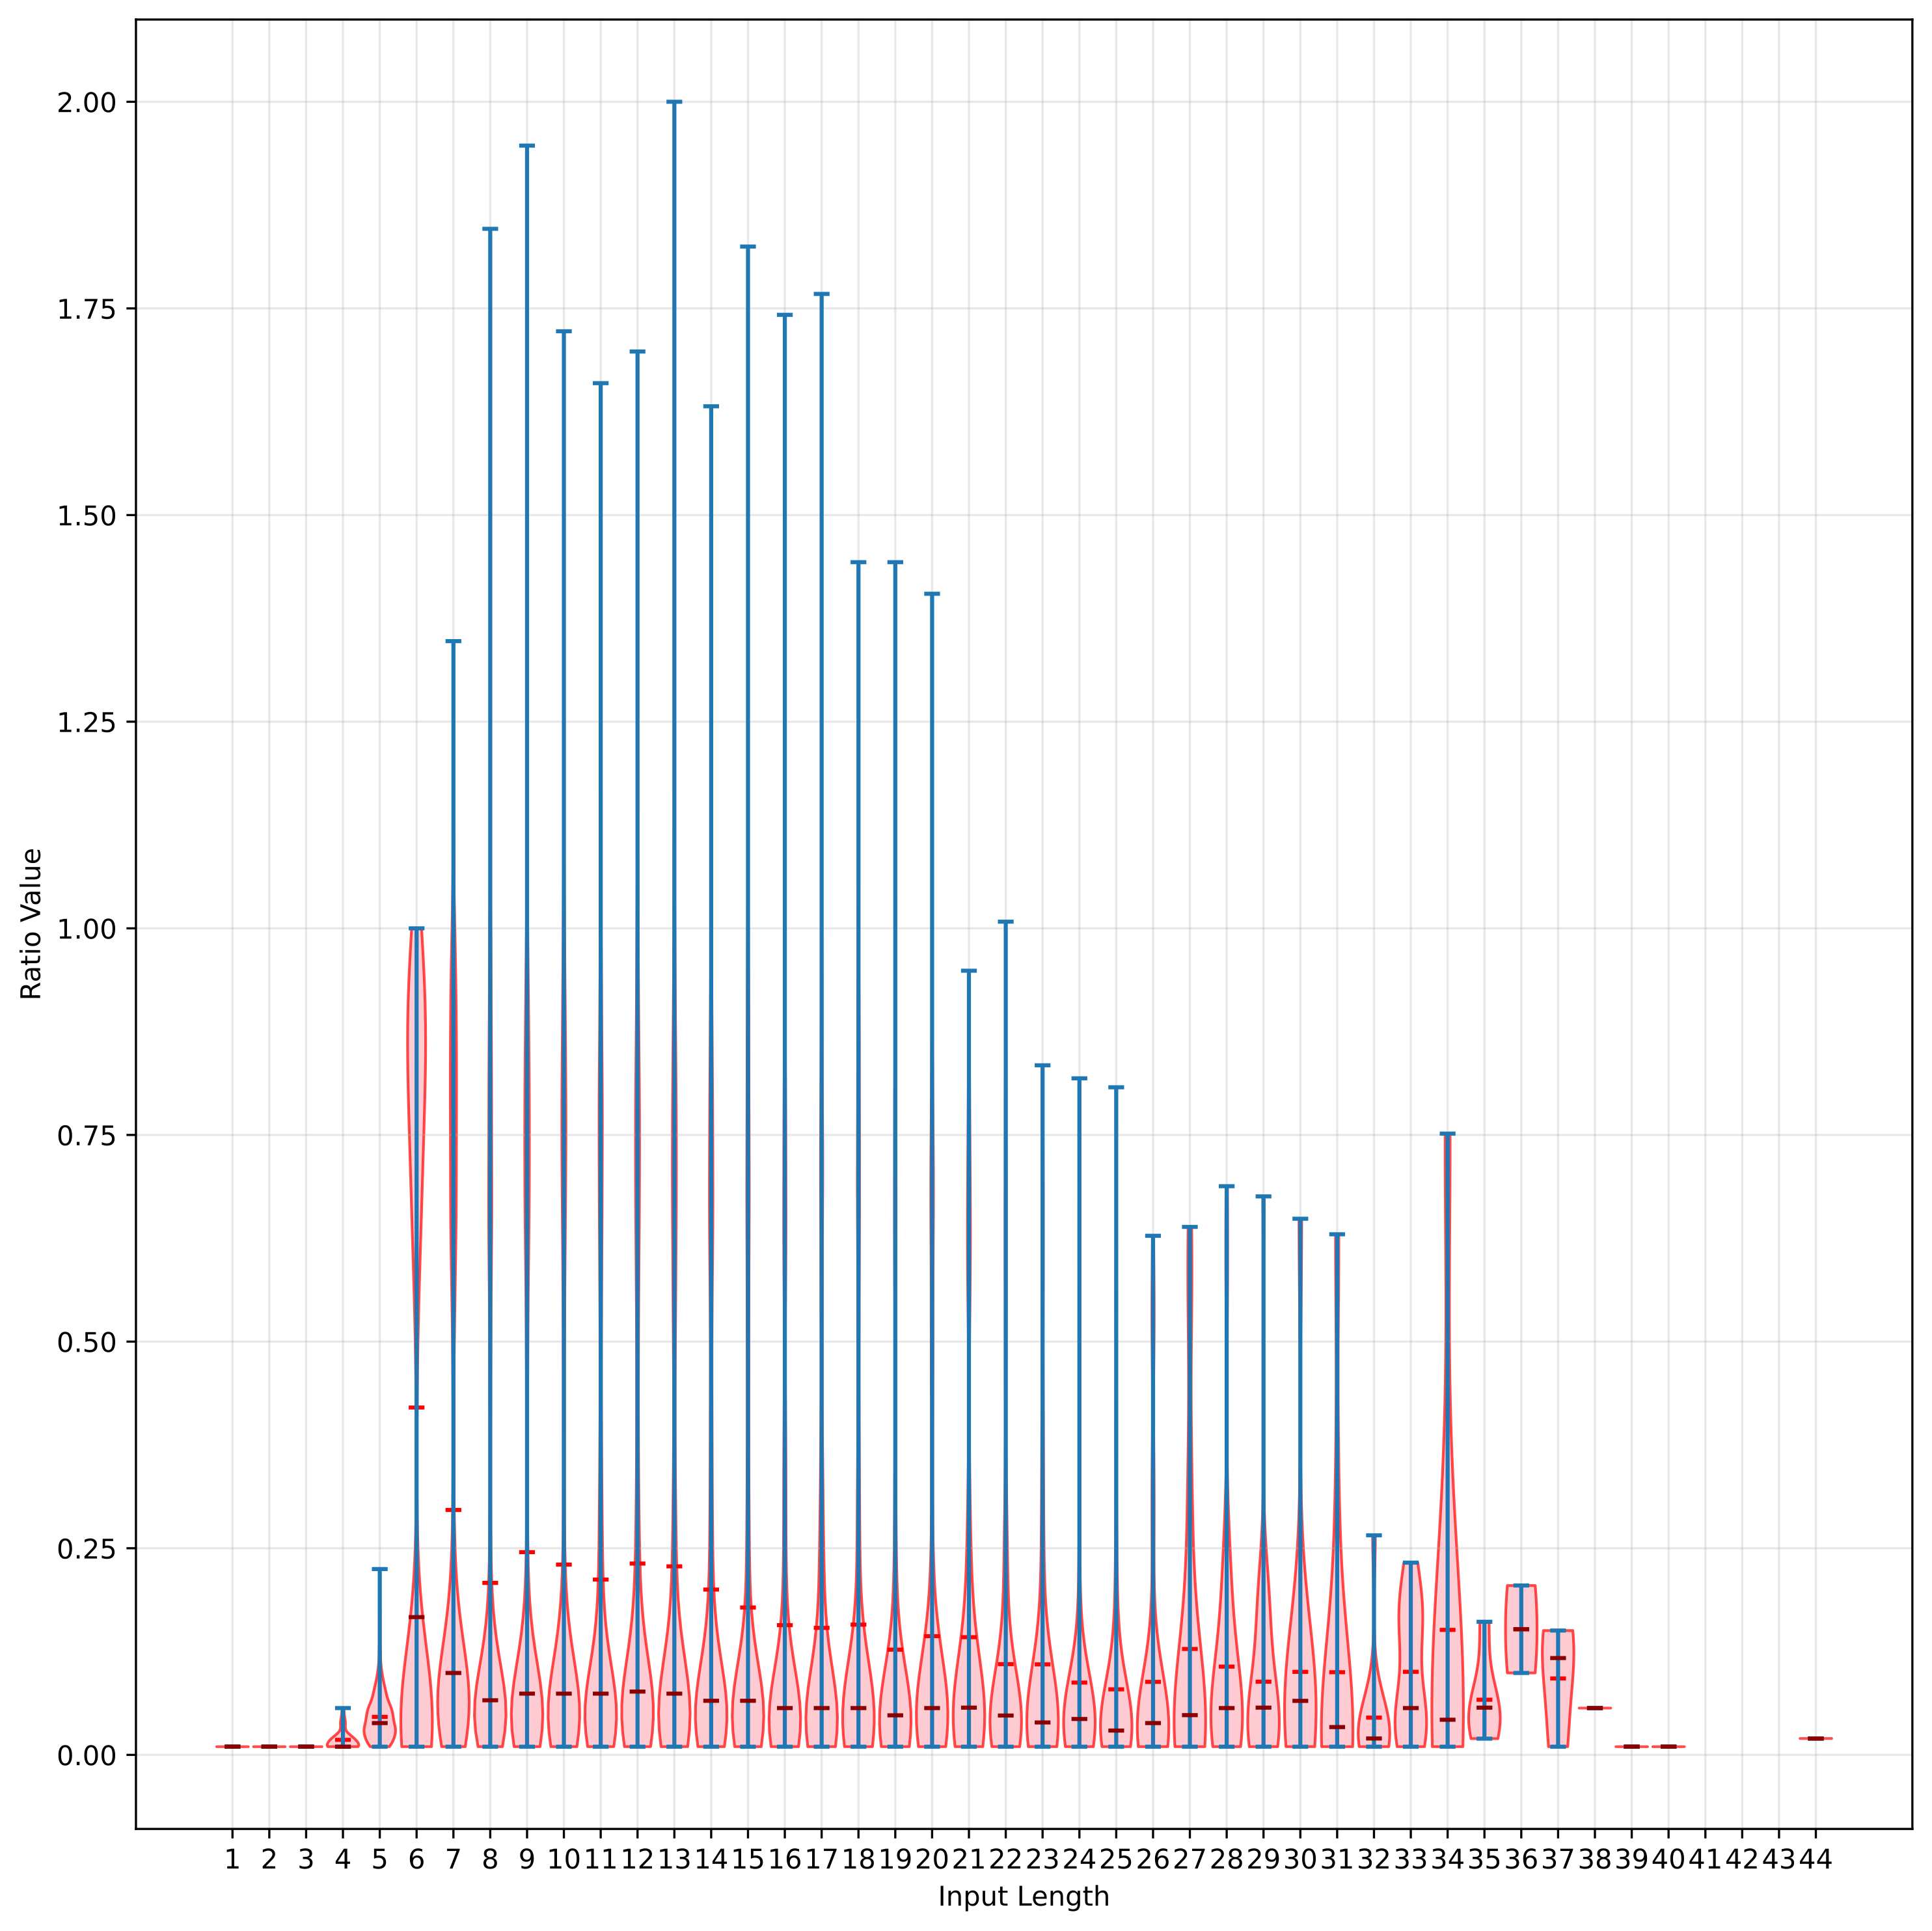
\includegraphics[width=\columnwidth]{assets/consistency/state-diff-violin.png}
  \caption{Ratio between incorrect and correct observer measurements across trace lengths when using state-diff feedback (violin width indicates density)}
  \label{fig:state-diff-inter-violin}
\end{figure}

\subsection{Throughput and Overcommit}
\label{Results:Overcommit}

\begin{figure}
  \makebox[\columnwidth]{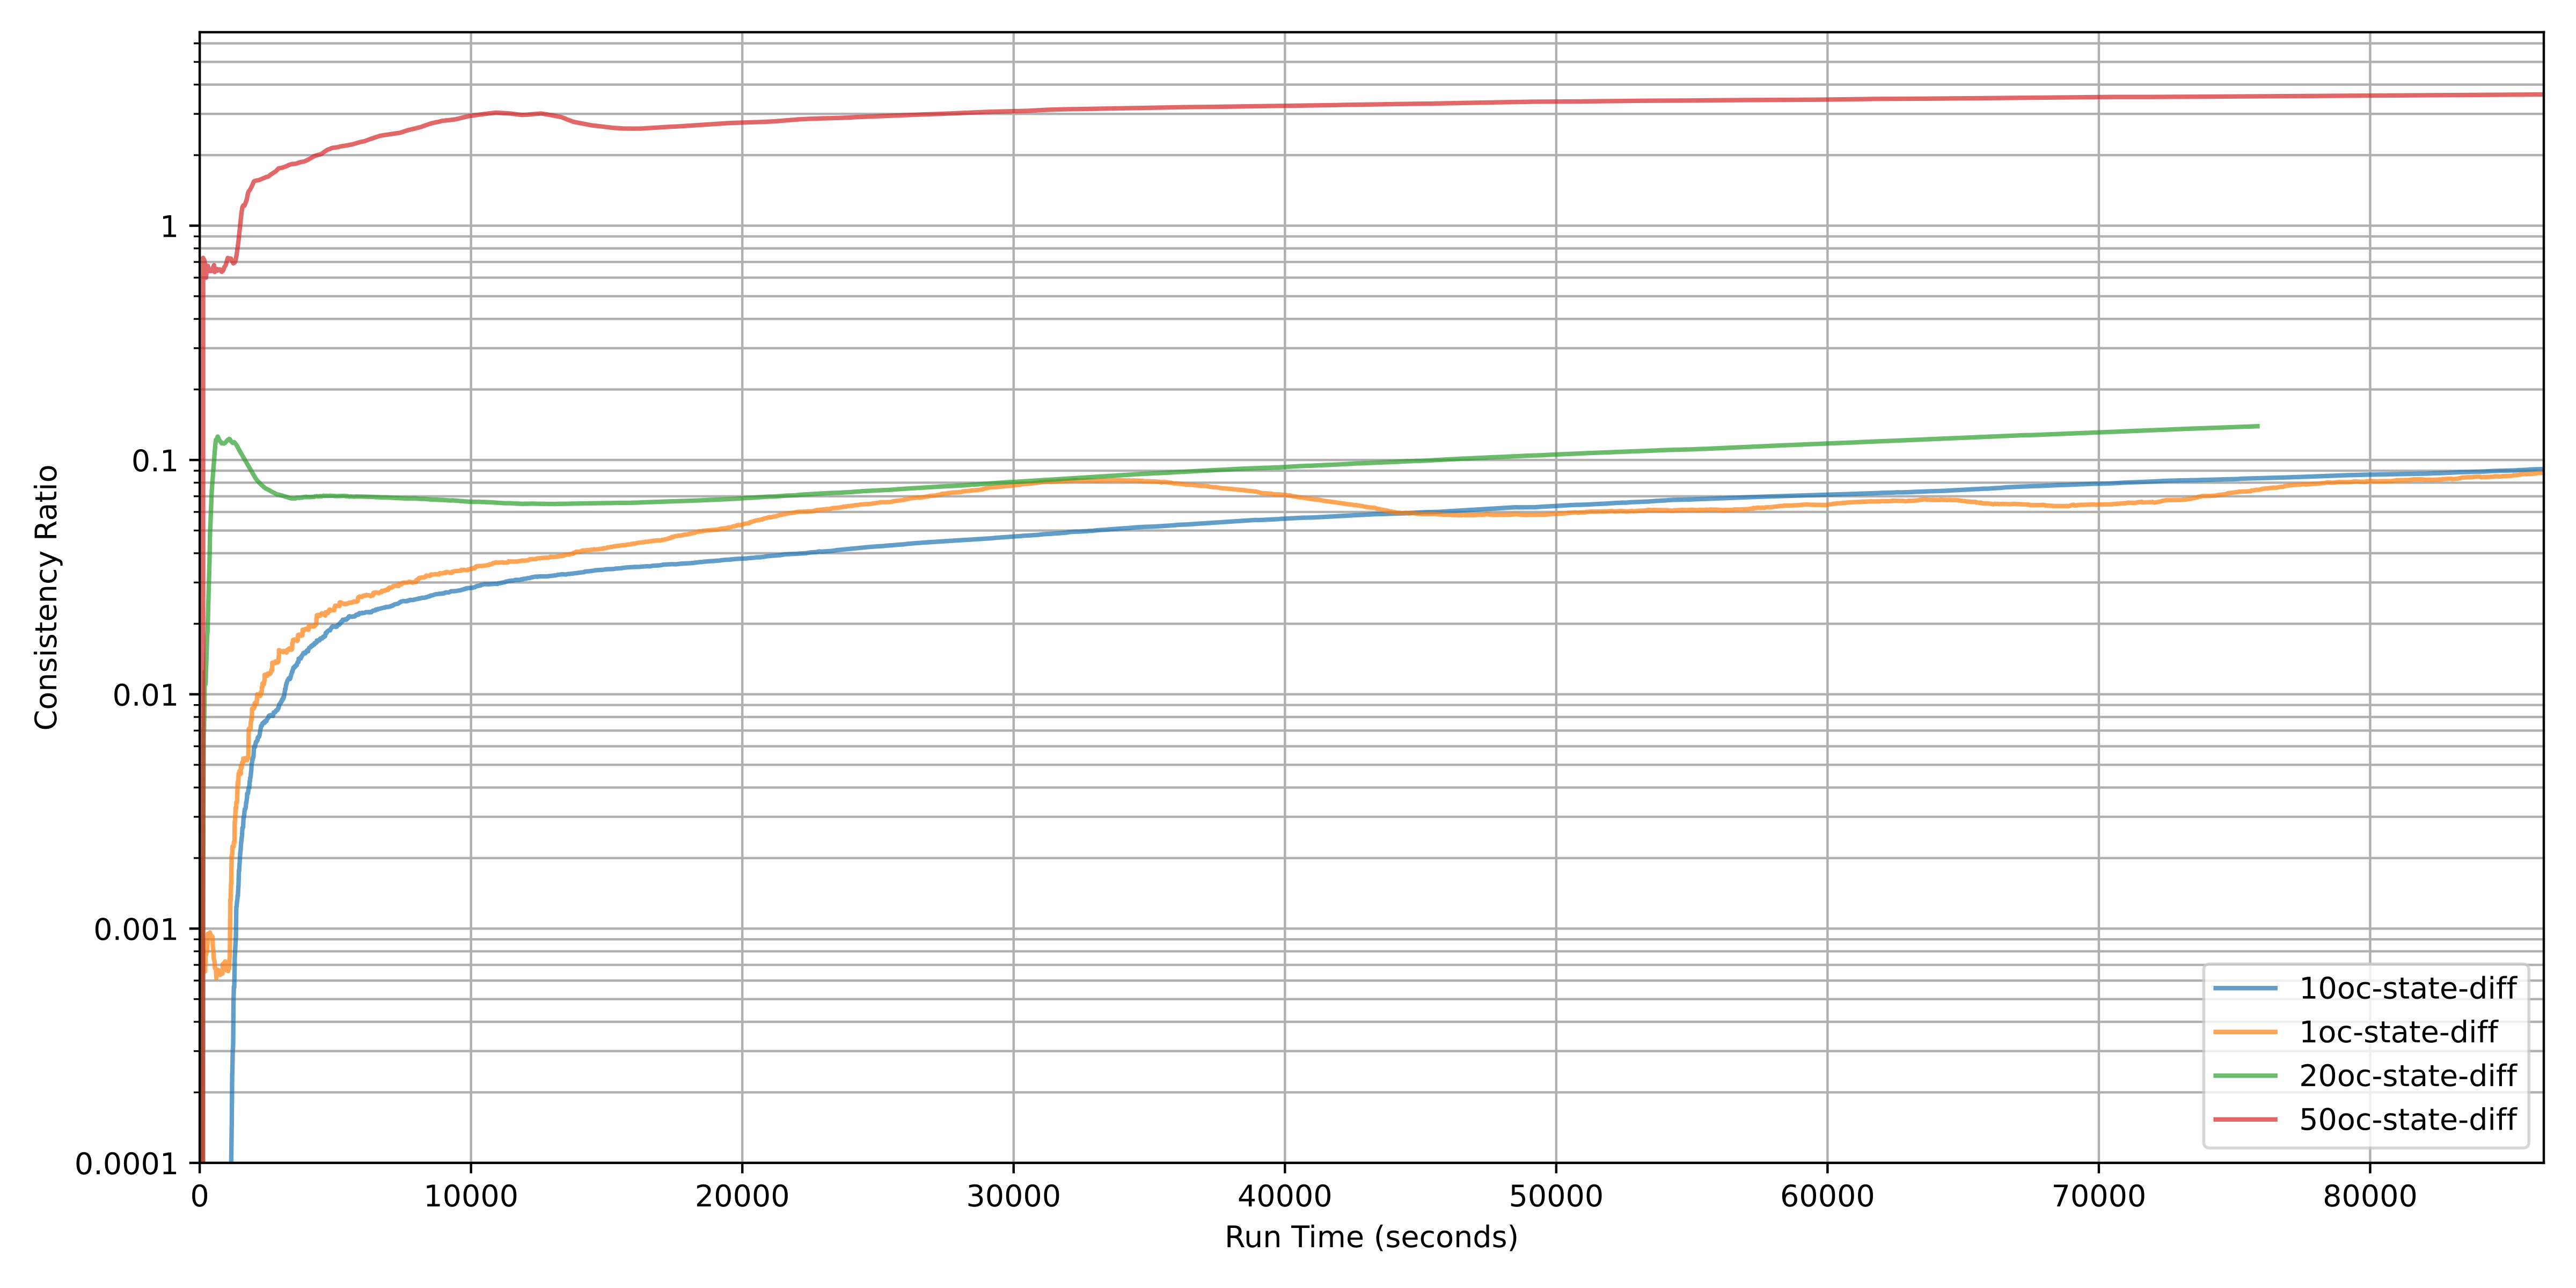
\includegraphics[width=1.1\columnwidth]{assets/throughput/all-other-to-most-rolling-avg-by-run_time-plot.png}}
  \todo{Add 50oc plot, limit}
  \caption{Consistencies across different overcommit values}
  \label{fig:overcommit-consistencies}
\end{figure}
\begin{figure}
  \makebox[\columnwidth]{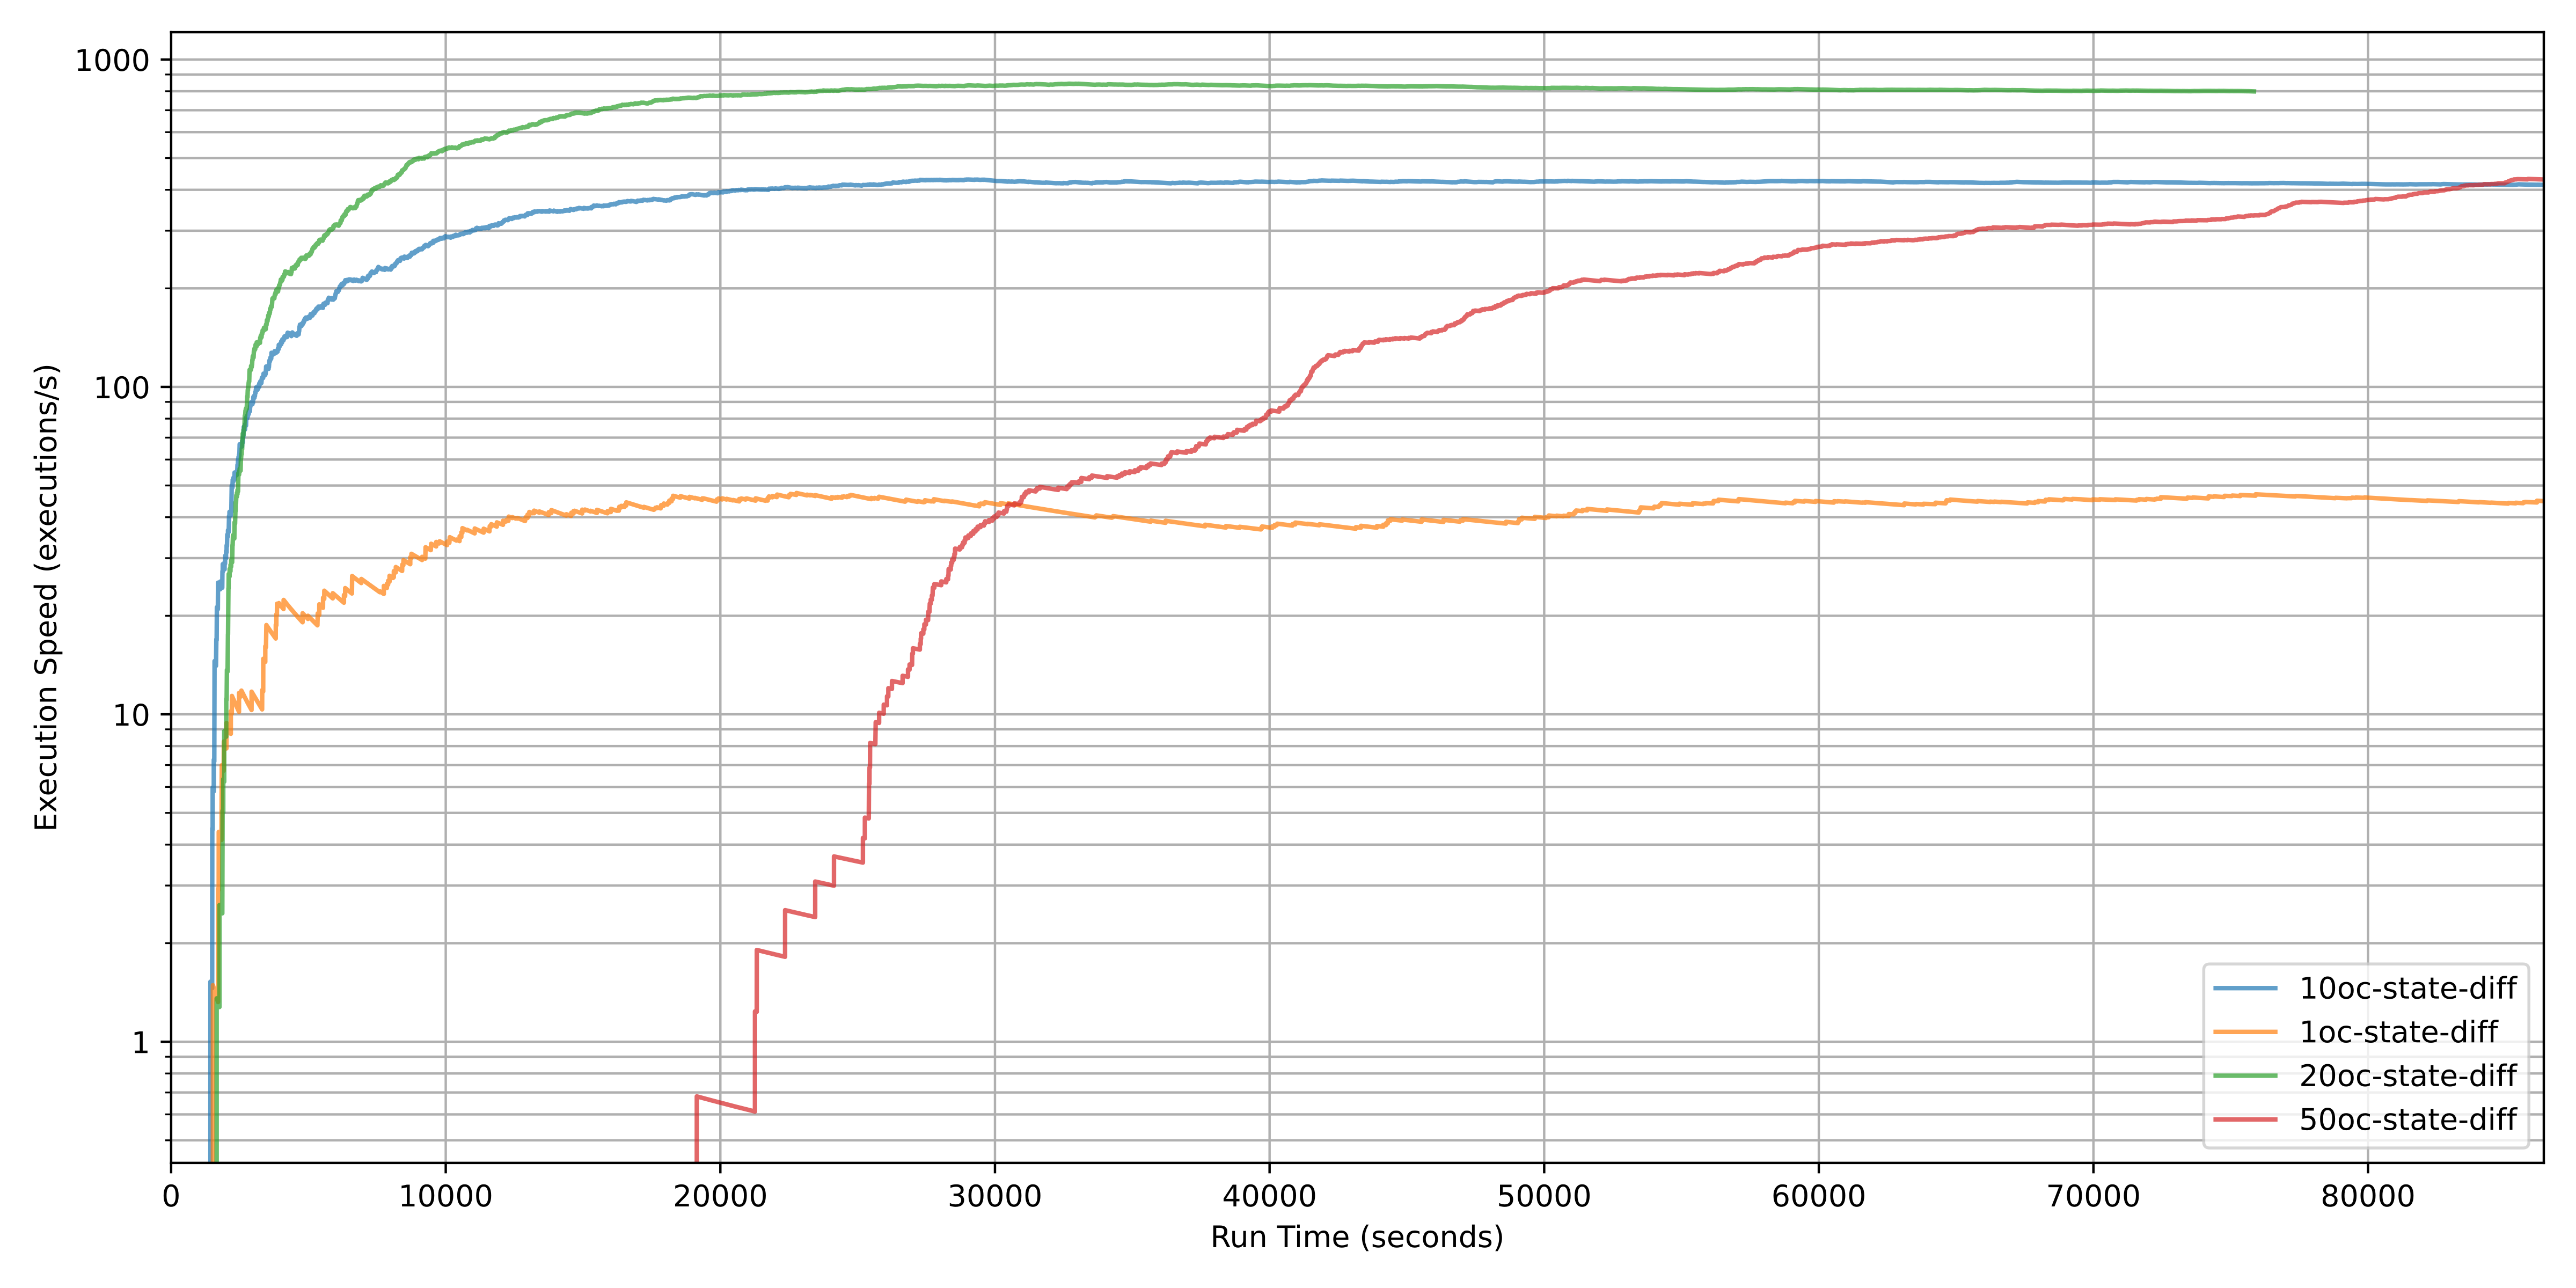
\includegraphics[width=1.1\columnwidth]{assets/throughput/exec-sec-by-run_time-plot.png}}
  \todo{Add 50oc plot, limit}
  \caption{Execution speed across different overcommit values}
  \label{fig:overcommit-exec-speed}
\end{figure}

When spawning a single fuzzing client per core, as is usual in fuzzing, the CPU time load averages approximately 0.8\% in user space and 1.9 in system space. Increasing the \code{overcommit} value and thus the number of clients per core increases instability rates for both observers, as seen in \cref{fig:overcommit-consistencies}. However, it simultaneously increases the overall execution speed of the fuzzer as seen in \cref{fig:overcommit-exec-speed}. The CPU loads for \code{overcommit} values of 10, 20, and 50 are 3.9\%/10.1\%, 8.7\%/23.1\%, and 8.3\%/89.9\% respectively.

\subsubsection*{Discussion}

As described in \cref{Implementation:ImplementationDetails:Client}, executing a single input on Zephyr leads to a dominating number wait states in both Zephyr and the fuzzer needed for synchronization. Increasing the number of clients per core does not fully load the CPU either, suggesting the limitation of \proj is scheduling over 2500 processes requiring precise timing for their execution consistency. There exists a tradeoff between speed and consistency when configuring \proj. Increased \code{overcommit} values and thus execution speed requires additional measures to mitigate the increased error rates. The primary such mitigation is additional repeated executions of the same input, which in turn slows down the overall execution speed with regard to the number of unique inputs evaluated. Since the error rates remain approximately consistent for \code{overcommit} values of up to 10, the remaining evaluations were done with \proj configured to run 10 clients per core.

\subsection{State Feedback vs. State-Diff Feedback}

\begin{figure*}[t]
  \centering
  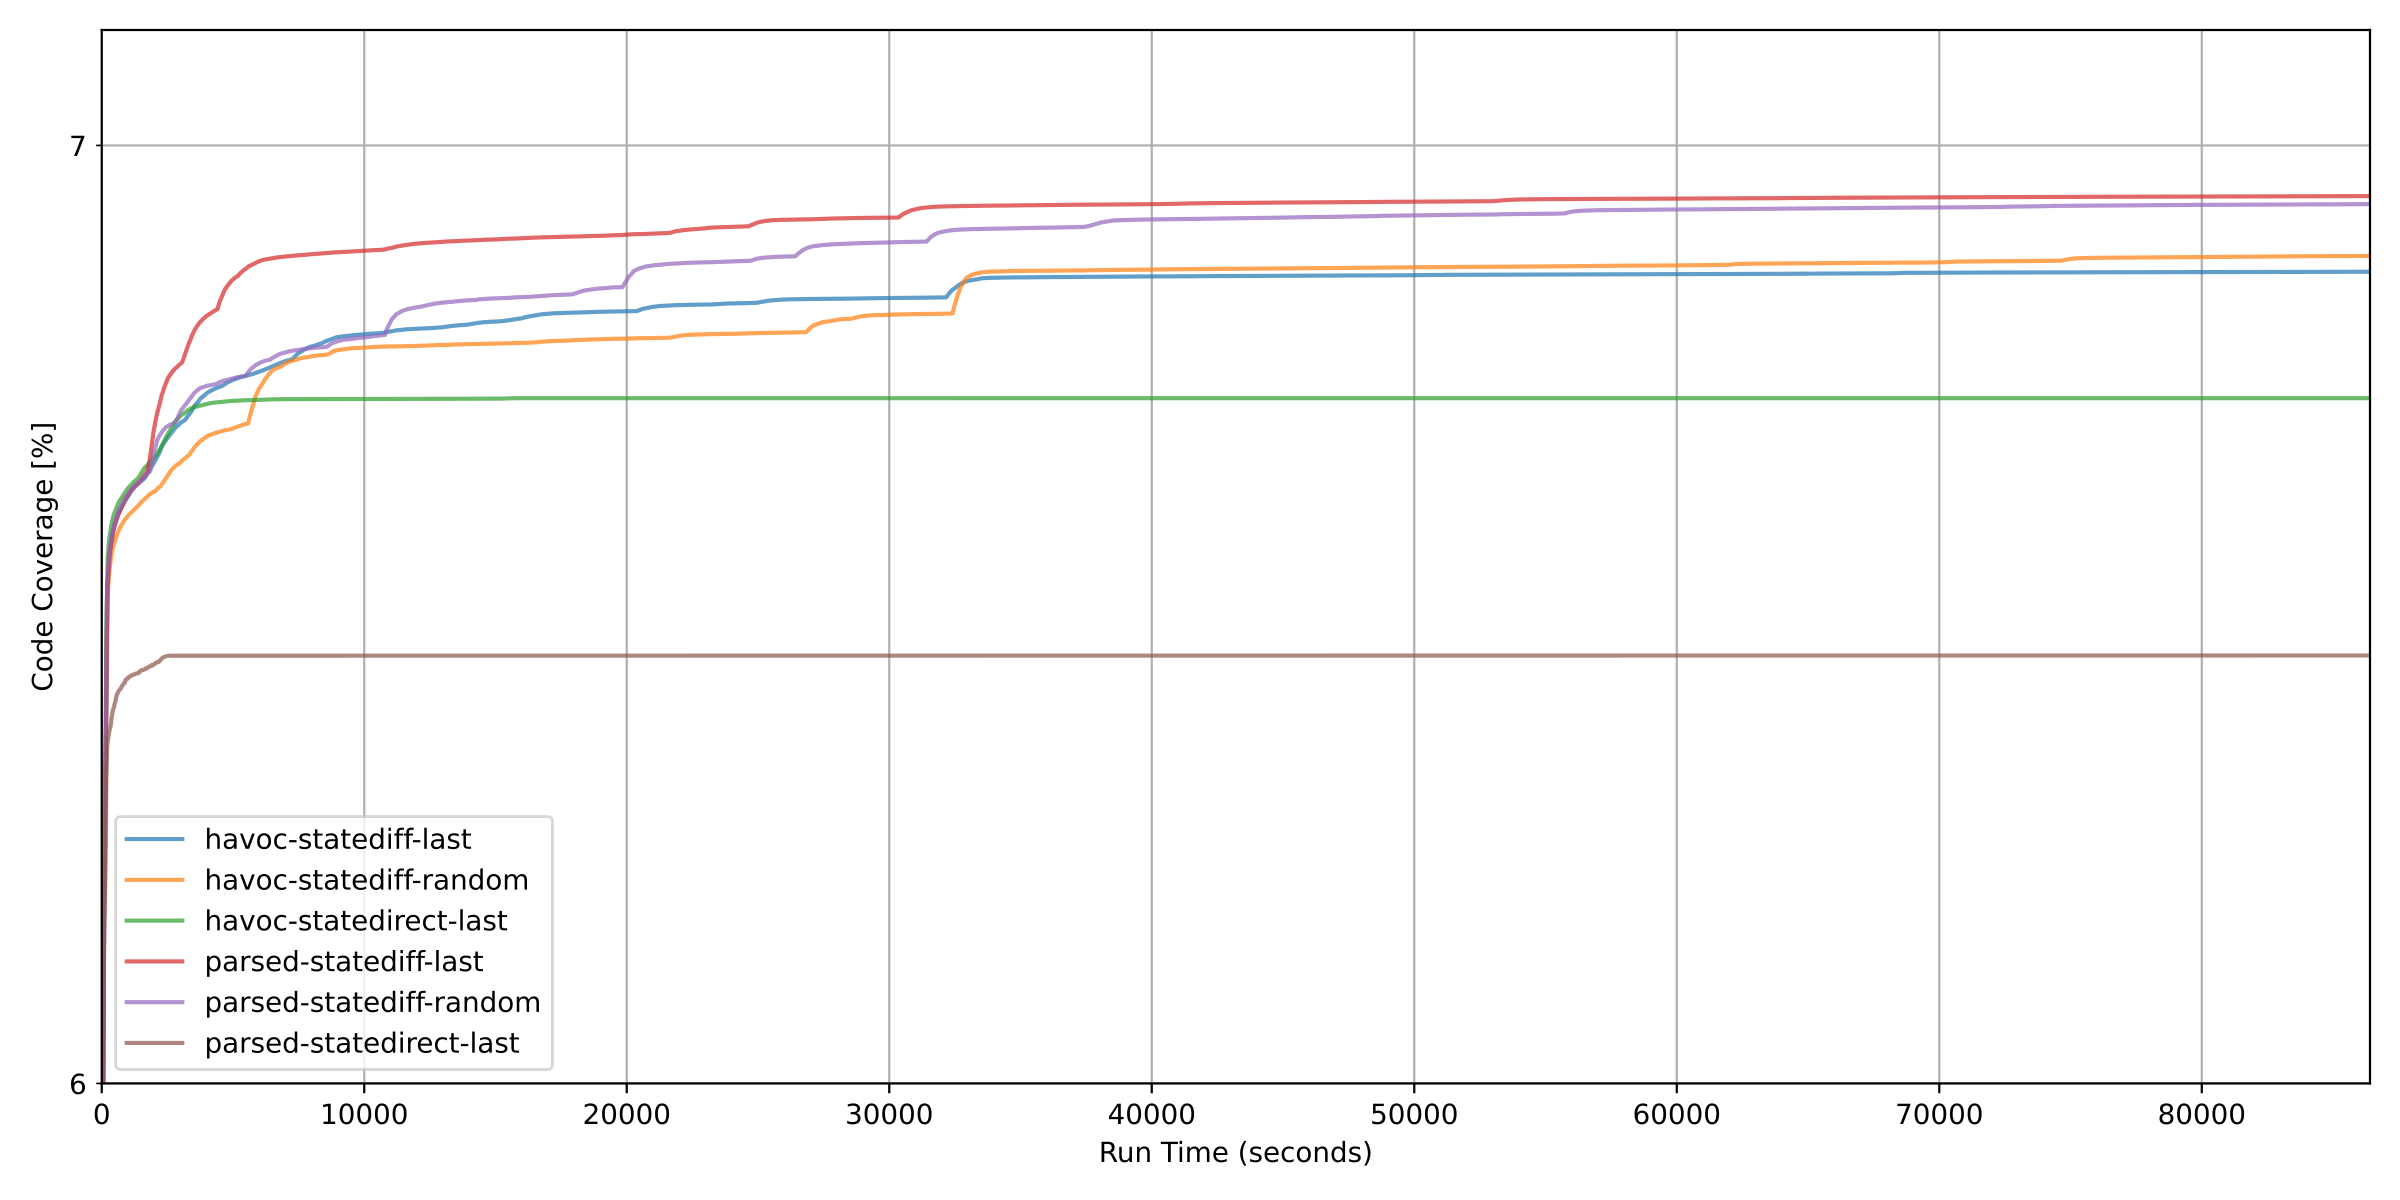
\includegraphics[width=0.9\textwidth]{assets/eval/coverage-observer-by-run_time-plot.png}
  \caption{Code coverage across different configurations}
  \label{fig:eval-cov}
\end{figure*}

\cref{fig:eval-cov} shows the coverage achieved by the different configurations of \proj. Note that \proj is configured to measure coverage across all parts of Zephyr, and is therefore unlikely to achieve code coverage of 100\%, as many parts of the logic are not currently examined by \proj. The most stark difference is between the configurations that rely on direct state feedback and those using state-diff feedback.

\begin{figure}
  \makebox[\columnwidth]{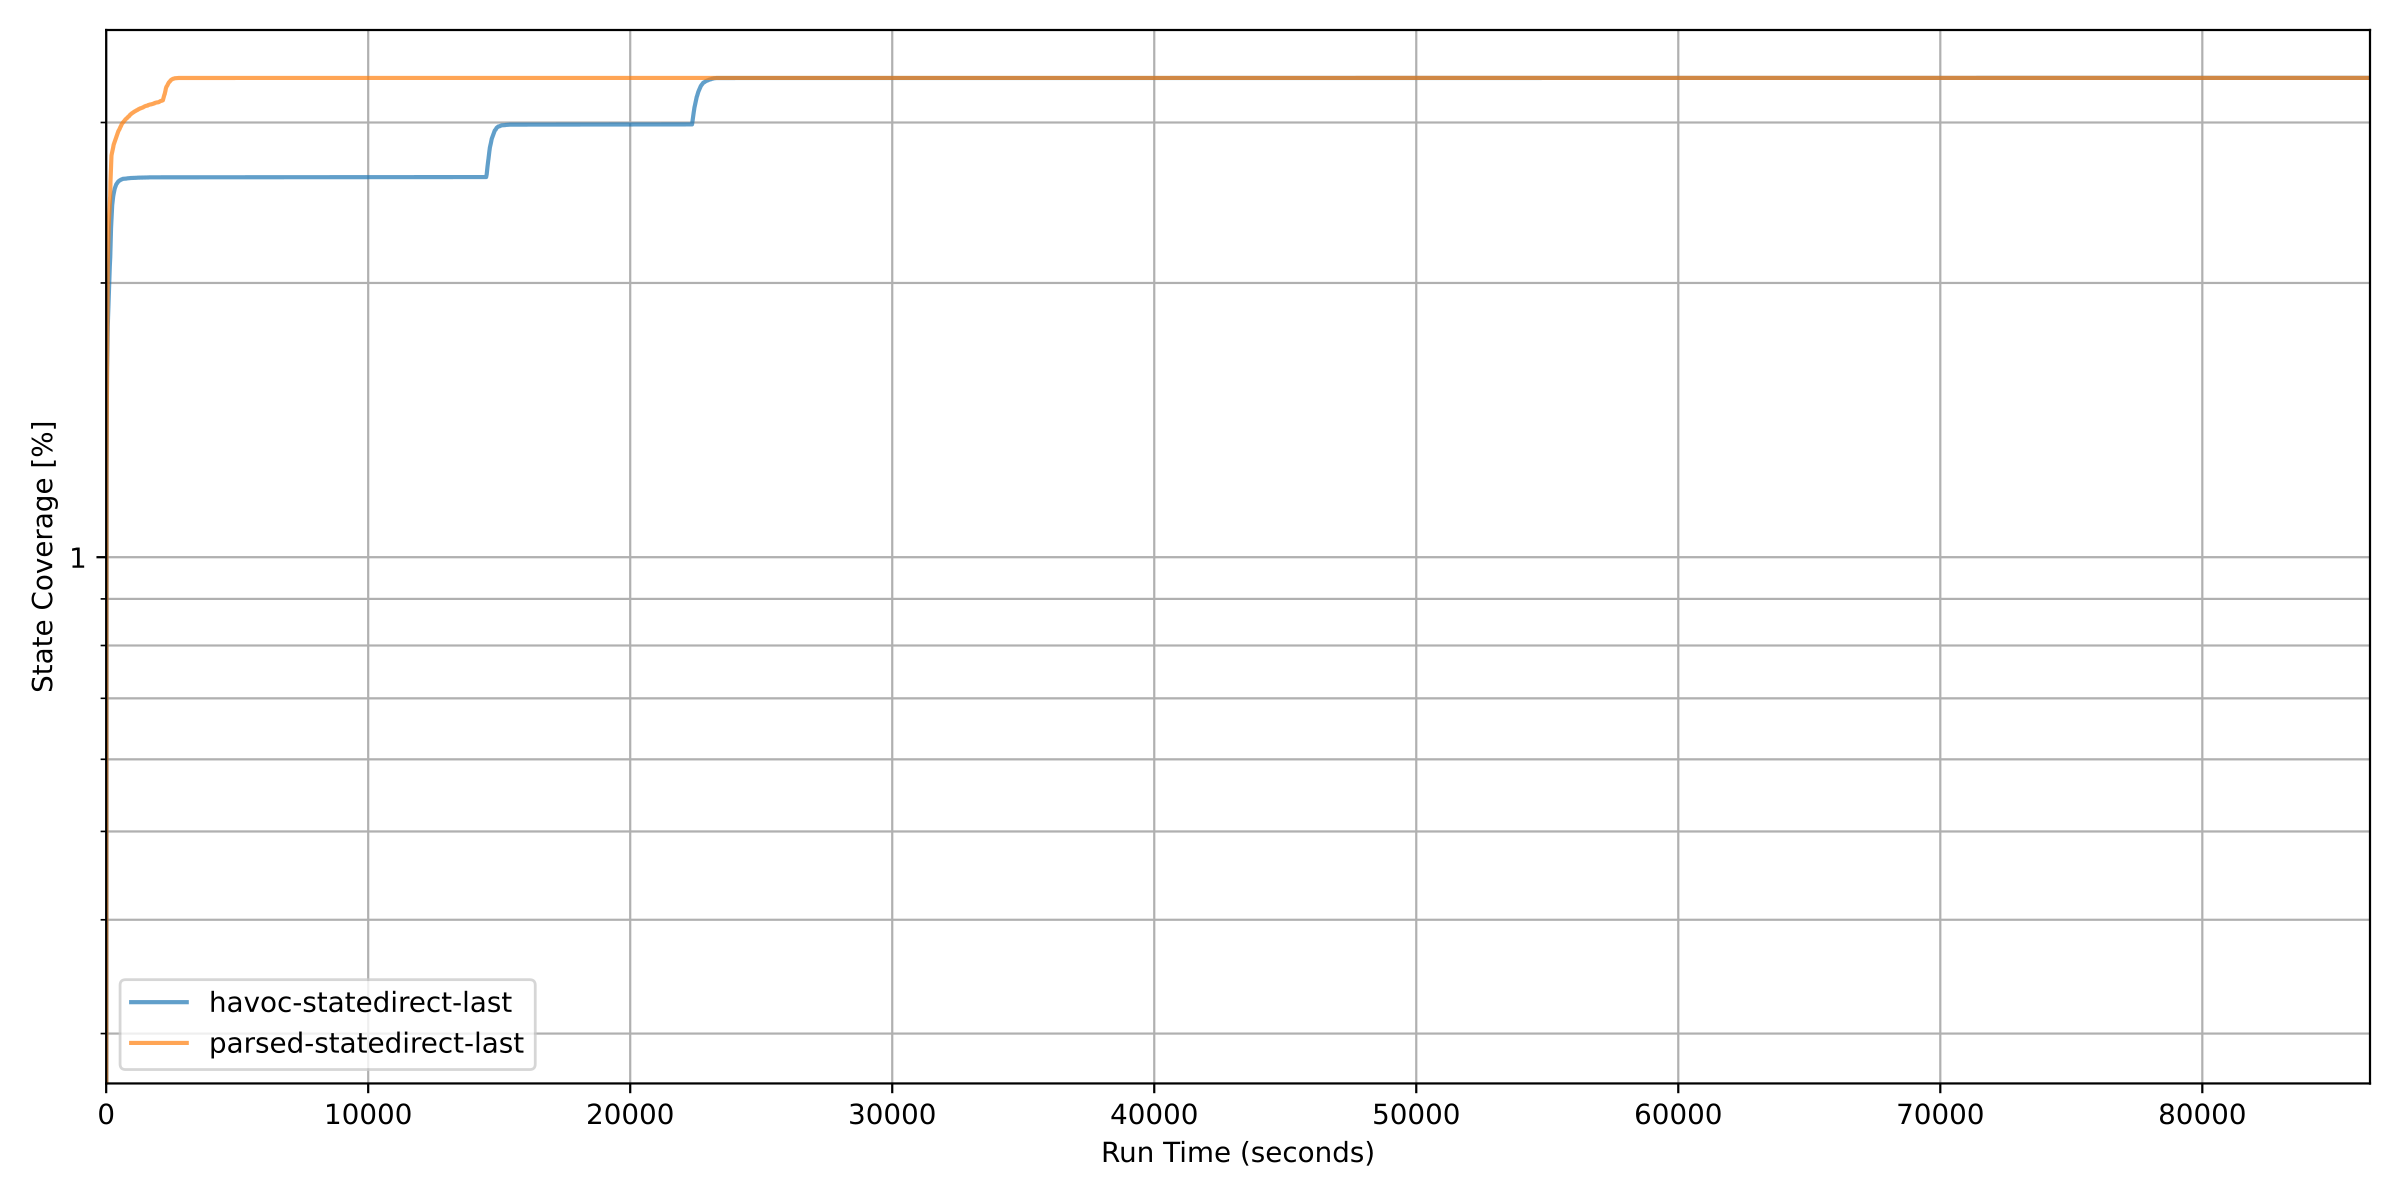
\includegraphics[width=1.1\columnwidth]{assets/eval/state-map-observer-by-run_time-plot.png}}
  \caption{States in replies recorded by \proj when configured using direct state feedback}
  \label{fig:eval-state-cov}
\end{figure}

\begin{figure}
  \makebox[\columnwidth]{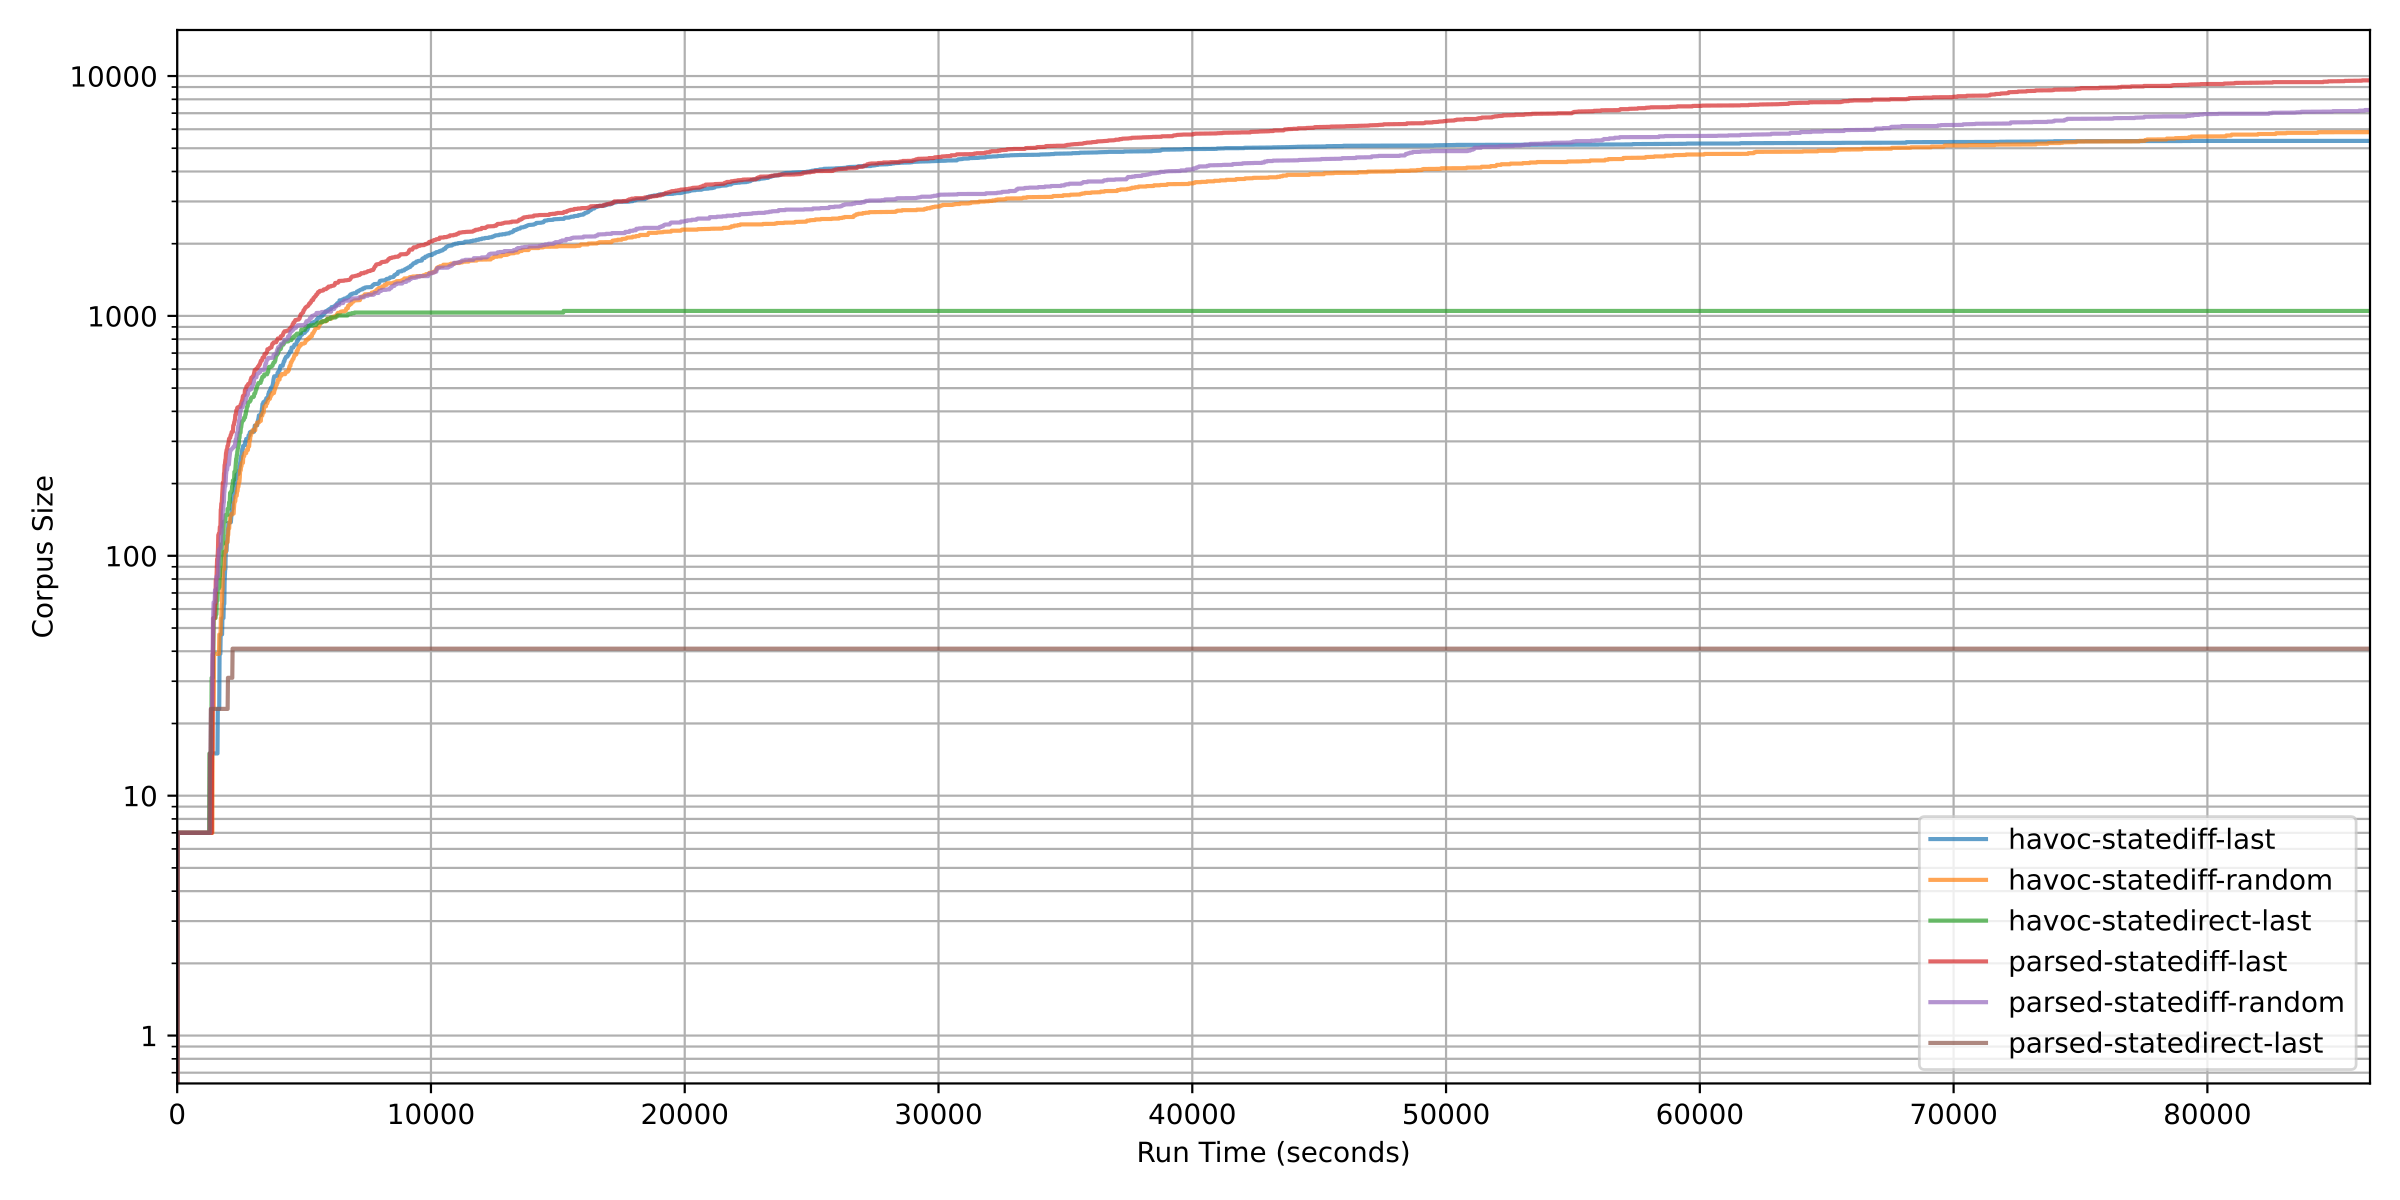
\includegraphics[width=1.1\columnwidth]{assets/eval/corpus-by-run_time-plot.png}}
  \caption{Number of corpus entries across different configurations}
  \label{fig:eval-corpus}
\end{figure}

\cref{fig:eval-state-cov} shows that \proj exhausts all achievable states within the first hours, including propagation to the found inputs to all 640 clients, and is unable to find any further improvements after that. Note that \proj is very unlikely to achieve a state coverage of 100\%, as Zephyr is not built to emit every combination of flags in the TCP header. \cref{fig:eval-corpus} further corroborates this by showing that no inputs are added to the corpus after that.

\subsubsection*{Discussion}

The number of states that can be emitted by Zephyr seems too small to make direct state feedback an effective feedback mechanism for \proj. It may however still improve a fuzzer if it is combined with another form of feedback, like code coverage. This was however not further evaluated due to the unreliability of coverage measurements in \proj (see \cref{Results:Consistency}).

\begin{figure}
  \makebox[\columnwidth]{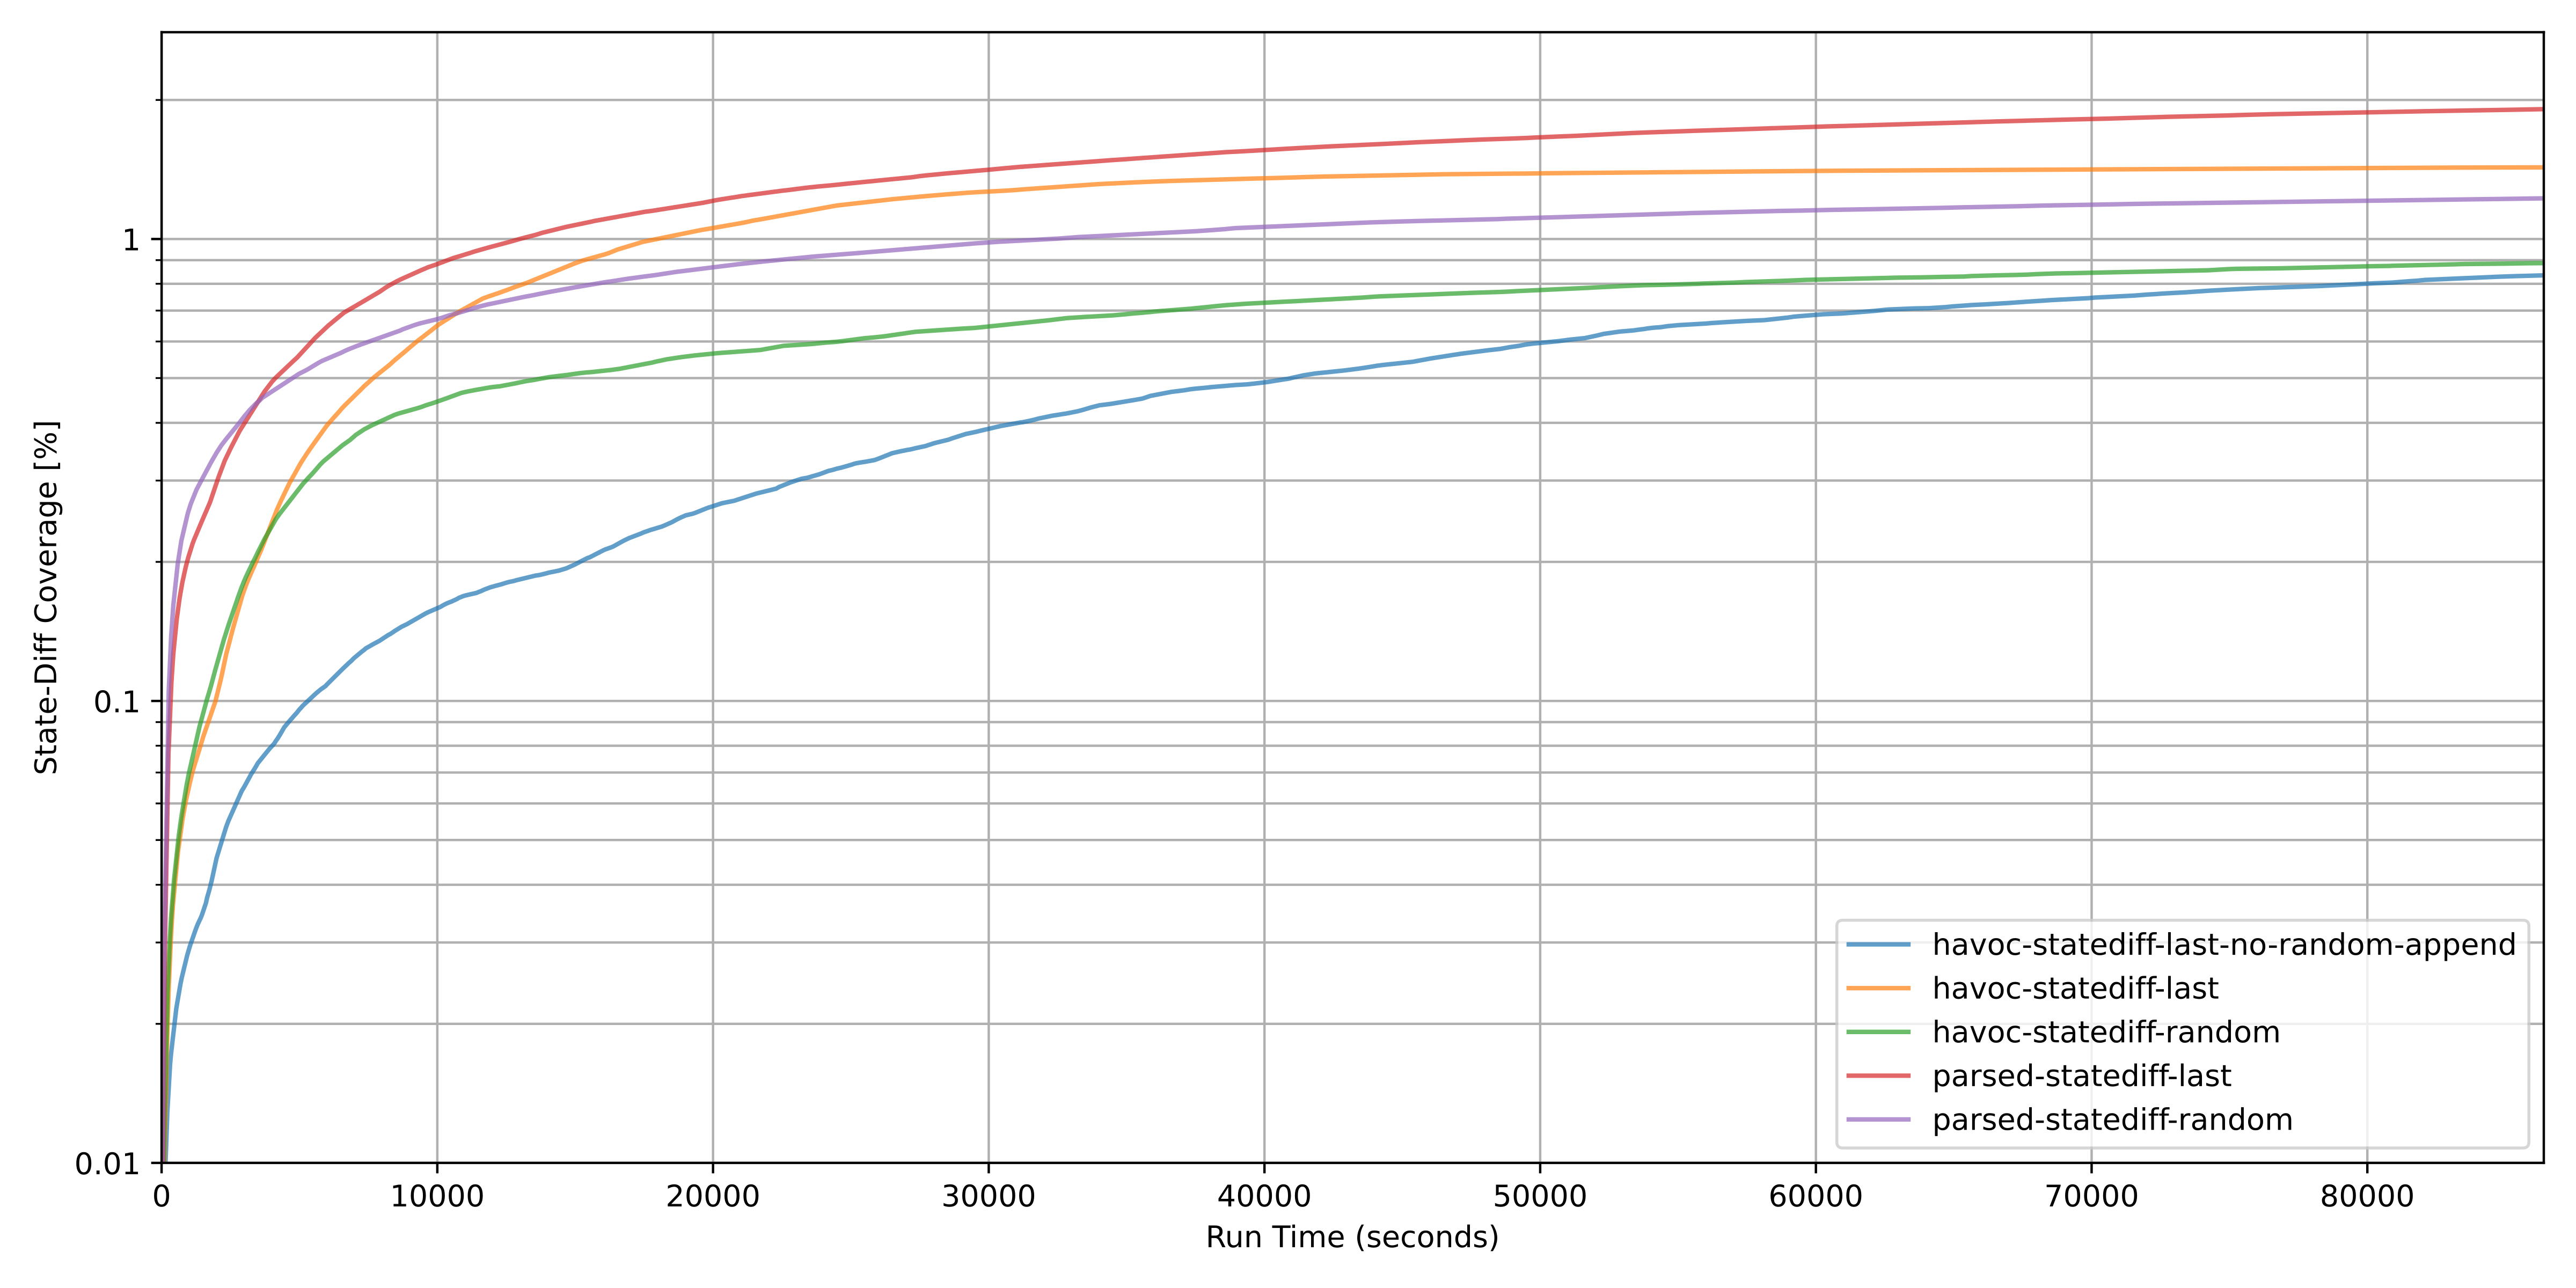
\includegraphics[width=1.1\columnwidth]{assets/eval/state-diff-map-observer-by-run_time-plot.png}}
  \caption{State-diff feedback covered by different configurations of \proj}
  \label{fig:eval-state-diff-map}
\end{figure}

\subsection{Mutation Target Selection}

\cref{Implementation:InputModelling:MutationTarget} introduced how \proj can be configured to mutate either a random message in a trace or always focus on the last message. \cref{fig:eval-cov} shows a small difference between the two options, for both byte array and parsed message representation. While the difference is larger in the early stages of the fuzzing campaign, selecting the last message as a mutation target is shown to be more effective even after 24 hours.

\cref{fig:eval-state-diff-map} further demonstrates that the strategy always mutating the last message is also more effective and efficient at covering all possible state-diff map entries.

\subsubsection*{Discussion}

When randomly selecting a message to mutate, \proj with a certain probability selects the last message, which may explain why after a while, it catches up to the alternative strategy of always mutating the last message. This further suggests that the assumption described in \cref{Implementation:InputModelling:MutationTarget} holds, and mutating early messages in long traces often renders the remainder of the trace useless, as the interdependencies between states and messages is broken.

\subsection{Input Modelling and Mutation}

\cref{fig:eval-cov,fig:eval-state-diff-map} show that modelling messages as a parsed data structure is more effective and efficient at maximizing code coverage and state-diff coverage.

\subsubsection*{Discussion}

When modelling messages as a parsed structure, \proj is severely limited in the possible input space it can explore. It can only output fixed layer 2 and 3 headers (except for their fields that depend on the packet contents), and even the TCP header always has a correct length field and checksum. However, these experiments show that this actually helps \proj to test more parts of Zephyr.

Byte array modelling of inputs and random mutation in theory is more powerful — it can generate inputs that invalidate only one of the fixed values listed above — it is very unlikely to randomly generate the correct values for all others. This further means that Zephyr will reject most packets generated by such mutation in its first parsing layer, while deeper logic is never reached. The additional logic reached by \proj in this configuration is exclusively due to the appending mutators, one of which will generate random valid TCP packets.\todo{proof}

%%%%%%%%%%%%%%%%%%%%%%%%%%%%%%%%%
%%% Conclusion %%%%%%%%%%%%%%%%%%
%%%%%%%%%%%%%%%%%%%%%%%%%%%%%%%%%

\section{Conclusion}
\label{Conclusion}
\subsection{Limitations and Future Work}

While this thesis presents a functional proof-of-concept fuzzer in \proj, as discussed in \cref{Results}, there remain a set of improvements to implement and questions it was unable to answer. First, sleep-interrupted busy waiting in both the fuzzer and Zephyr could be replaced by a form of kernel-supplied synchronization technique such as semaphores. There further is a list of efficiency improvements, such as incremental packet parsing, that were not completed because \proj is not primarily constrained by CPU load but instead consistency.

First, prior work has shown that the seeds used in a fuzzer have a significant impact on the fuzzer's performance\cite{Seeding}. \proj currently relies on subsets of a single recorded interaction, which could be extended with other traces, specifically those exercising different paths through the state machine, such as cancelled or otherwise incomplete interactions may prove beneficial for \proj's performance.

Additional seeding could further improve the range of packets supported by the fuzzer: Support for TCP over IPv6 would require only little additional engineering in combination with additional seeds. Similarly, options in the different protocol headers (see \cref{Background:TcpIsStructured}) are currently only partially fuzzed when using parsed input structures, which could be improved by additional seeds in addition to a list of additional mutators.

TCP-Fuzz\cite{TCPFuzz} correctly identified that TCP/IP stacks have an input space larger than that of the packets they process in their configuration and invocation through system calls (see \cref{RelatedWorks:InputModelling}). These are currently not mutated in \proj but instead fixed to the configuration of the \code{sockets/echo} sample (see \cref{Implementation}).

\proj further could be used a basis to fuzz other protocols at different networking layers, such as application layer protocol implementations of an FTP or SMTP server or additional transport layer protocols like QUIC. This may further allow comparison between \proj and previous work on these protocols (refer to \cref{RelatedWorks:ProtocolFuzzing}).

However, the same challenges as outlined in \cref{RelatedWorks:ProtocolFuzzing:TargetDifferences} remain. Comparing \proj to other approaches would either require reengineering other fuzzer's target interaction to be compatible with Zephyr, or extracting the improvements made by \proj and build a fuzzer around them targeting other code. Improvements made to LibAFL would make protocol fuzzing in general easier, but it still requires setting up the appropriate parsed data structured and mutators. However, this work could further confirm the results described in \cref{Results} independent of Zephyr or TCP/IP.

Alternatively, \proj could be evaluated on other implementations of TCP/IP stacks, such as userland implementations (\cref{Implementation:ImplementationDetails:HelperFunctionality} discusses how one such implementation is already partially integrated into \proj), or the network stacks of other OSs. The main challenge in this is the adaptation of the target similar to what is described in \cref{Implementation}, such as sanitizer and code coverage instrumentation and drivers for the shared memory-based pseudo-networking or an alternate way of exchanging packets. Access to alternate implementations would also allow \proj to implement differential fuzzing, testing the behavior of the different targets against each other to find logic errors that do not corrupt the memory and thus cannot currently be found by \proj.

Finally, one could investigate how state information could be used besides feedback. \cref{RelatedWorks:ProtocolFuzzing:UseOfState} discusses advancements other projects have shown by using state information in other parts of the fuzzer, such as the scheduler.

\subsection{Contributions and Summary}
This thesis presents \proj, a proof-of-concept fuzzer targeting the TCP/IP stack of Zephyr. To achieve this, it introduces a custom ethernet driver based on shared memory to reduce host kernel dependencies. \code{native_sim}, the environment simulation wrapper, is used to run Zephyr without the need for a dynamic emulation layer. It is built on and extends the fuzzing framework LibAFL.

In addition to initial investigation into the reasons for Zephyr's at times unpredictable behavior, I evaluated the differences in performance of mutations on serialized and parsed packet representations, two strategies to select which message in a trace to mutate, and two heuristics to estimate the TCP state of a connection based on returned packets.

The experiments show that even limited structure-aware mutation is more efficient at covering both code coverage and the state space compared to naïve random mutation. In addition to appending new packets, mutating the last message of a trace is more efficient than selecting a random message to mutate. Finally, I present that maximizing simple state feedback as calculated by the heuristic quickly saturates the possible state space after which \proj no longer makes any progress. Conversely, maximizing coverage across state transitions proofs to be more effective.

\vspace*{\stretch{2}}
\begin{center}
  \centering
  In the interest of open science, the source code and all artifacts produced during this project are publicly available and released under an open-source license. During development, thousands of lines of code have been introduced to multiple upstream projects. All artifacts produced for this project are available at

  \vspace{8px}

  \href{https://github.com/riesentoaster/fuzzing-zephyr-network-stack}{github.com/riesentoaster/fuzzing-zephyr-network-stack}.\todo{change url}
\end{center}
\vspace*{\stretch{1}}

\onecolumn
\newpage
\twocolumn

\defbibheading{bibliography}[\bibname]{\section*{#1}}
\addcontentsline{toc}{section}{\bibname}
\printbibliography

\end{document}